%% LyX 1.3 created this file.  For more info, see http://www.lyx.org/.
%% Do not edit unless you really know what you are doing.
\documentclass[oneside,english,useAMS, usenatbib]{mn2e}
%\usepackage[T1]{fontenc}
%\usepackage[latin1]{inputenc}
\setcounter{tocdepth}{3}
\usepackage{graphicx}
\usepackage{amssymb}

\makeatletter

%%%%%%%%%%%%%%%%%%%%%%%%%%%%%% LyX specific LaTeX commands.
%% Bold symbol macro for standard LaTeX users
\newcommand{\boldsymbol}[1]{\mbox{\boldmath $#1$}}

%% Because html converters don't know tabularnewline
\providecommand{\tabularnewline}{\\}

%%%%%%%%%%%%%%%%%%%%%%%%%%%%%% User specified LaTeX commands.
\usepackage{times}

\newcommand{\aap}{A\&A}
\newcommand{\aaps}{A\&AS}
\newcommand{\apj}{ApJ}
\newcommand{\apjl}{\apj}
\newcommand{\pasp}{PASP}
\newcommand{\aj}{AJ}
\newcommand{\mnras}{MNRAS}
\newcommand{\apjs}{ApJS}
\newcommand{\aapr}{A\&AR}
\newcommand{\pasj}{PASJ}

\newcommand{\kmps}{\mathrm{km~s^{-1}}}
\newcommand\ion[2]{#1$\,${\sc {#2}}}   % ion, i.e., CII = \ion{C}{ii}
\newcommand{\Kelvin}{\mathrm{K}}

\usepackage{babel}
\makeatother
\begin{document}
\title[On the formation of H$\alpha$ around classical T Tauri stars]{On the formation of H$\alpha$ around classical T Tauri stars}

\author[R. Kurosawa et\,al.]{Ryuichi Kurosawa$^1$\thanks{E-mail: rk@astro.ex.ac.uk}, Tim J. Harries$^1$ and Neil H. Symington$^2$\\
$^1$School of Physics, University of Exeter, Stocker Road, Exeter EX4 4QL. \\
$^2$School of Physics and Astronomy, University of St. Andrews, North Haugh, St. Andrews, Fife, KY16 9SS.}

\date{Dates to be inserted}

\pagerange{\pageref{firstpage}--\pageref{lastpage}} \pubyear{2005}

\maketitle

\label{firstpage}

\begin{abstract}

We present  radiative transfer models of classical T~Tauri stars, and investigate the formation of H$\alpha$
in order to understand their complex circumstellar environment, and to explain
the wide variety of emission line profiles seen in observations. To
overcome the limited applicability of the radiative transfer models
with only magnetospherical accretion to fitting observed H$\alpha$
profiles, and to any other lines affected by the stellar wind) presented,
two types of kinematic wind models are introduced: (1)~the bipolar
wind model in which the wind is originated from the star itself, and
(2)~the disc-wind model in which the wind originates from the inner
part of the accretion disc. We perform systematic investigations of
the model parameters for the wind and the magnetosphere to search
for possible geometrical and physical conditions which lead to the
types of profiles seen in observations. We find both wind models
can reproduce the wide range profile types seen is observations, 
although the inclination dependence of the line equivalent width
predicted by the bipolar wind model agree with trends seen in the
observation, but the disc-wind model does not. Using the model results,
we examine the H$\alpha$ spectroscopic classification used by Reipurth
et.~al , and discuss the basic physical conditions required to reproduce
the profiles in each classified type. Using the hybrid model, we fit
the observed H$\alpha$ from the optical component of T~Tau triple
system (T~Tau~N), and find its ratio of the mass-loss to mass-accretion
rate to be $\sim0.18$ with the cold ($T_{\mathrm{wind}}\approx8000\,\mathrm{K}$)
bipolar wind model .

\end{abstract}

\begin{keywords}
stars: formation -- circumstellar matter -- radiative transfer -- stars: pre-main-sequence
\end{keywords}


\section{Introduction }

\label{sec:Introduction}

T~Tauri stars (TTS) are young ($<\sim3\times10^{6}\,\mathrm{yrs}$,
\citealt{appenzeller:1989}) low-mass stars, and are the progenitors
of solar-type stars. Classical T~Tauri stars (CTTS) exhibit strong
H$\alpha$ emission, and typically have spectral types of F--K. Some
of the most active CTTS show emission in higher Balmer lines and metal
lines (e.g., \ion{Ca}{ii}~H and K). They also exhibit an excess
amount of continuum flux in the ultraviolet (UV) and infrared (IR).
Their spectral energy distribution and polarisation data suggest the
presence of a circumstellar disc, which plays an important role in
regulating dynamics of gas flows around CTTS.

Many observational studies (e.g., \citealt{herbig:1962}; \citealt{edwards:1994};
\citealt{kenyon:1994}; \citealt{reipurth:1996}; \citealt{alencar:2000})
of CTTS line profiles show evidence for both outward wind flows and
inward accretion flows, as seen in the blue-shifted absorption features
in H$\alpha$ profiles and the redshifted inverse P~Cygni (IPC) profiles
respectively. Typical mass-loss rates of CTTS are about $10^{-9}\,\mathrm{M_{\sun}\, yr^{-1}}$
to $10^{-7}\,\mathrm{M_{\sun}\, yr^{-1}}$ (e.g., \citealt{kuhi:1964};
\citealt{edwards:1987}; \citealt{hartigan:1995}), and the mass-accretion
rates are also about $10^{-9}\,\mathrm{M_{\sun}\, yr^{-1}}$ to $10^{-7}\,\mathrm{M_{\sun}\, yr^{-1}}$
(e.g., \citealt{kenyon:1987}; \citealt*{bertout:1988}; \citealt{gullbring:1998}).
Recent H$\alpha$ spectro-astrometric observations by \citet{takami:2003}
show the direct evidence for the presence of bipolar and monopolar
outflows down to $\sim1\,\mathrm{AU}$ scale (e.g.\,CS~Cha and RU~Lup).
Similarly, ESO VLT observation of high-resolution ($R=50\,000$)
two-dimensional spectra of edge-on CTTS (HH30$^{*}$, HK~Tau~B,
and HV~Tau~C) by \citet{appenzeller:2005} show the extended H$\alpha$
emission in the direction perpendicular to the obscuring circumstellar
disc, and in both above and below the disc --- suggesting the presence
of the bipolar outflows. On a larger scale, \emph{HST} observation
of HH30 \citet{burrows:1996} shows the jet traced to within $\lesssim30$~AU
from the star. The jet has a cone shape with an opening angle of $3^{\circ}$
between 70 and 700 AU \citep{koenigl:2000}. \citet{alencar:2000}
found about 80 per cent of their samples (30 CTTS) show blue-shifted
absorption components in at least one of Balmer lines and Ca~K (most
commonly in H$\alpha$). 

In the currently favoured model of accretion flows around CTTS, the
accretion discs are disrupted by the magnetosphere of stars which
channels the gas from the disc onto the surface of the stars (e.g.,
\citealt{uchida:1985}; \citealt{koenigl:1991}; \citealt{cameron:1993};
\citealt{shu:1994}). This picture of the accretion flows is supported
by the evidences that CTTS have relatively strong ($\sim10^{3}\mathrm{G}$)
magnetic field (e.g., \citealt*{jonhs-krull:1999}; \citealt{guenther:1996})
and by the radiative transfer models which reproduce the observed
profiles for some TTS (\citealt{muzerolle:2001}). The magnetospherical
accretion model naturally explains the blue-ward asymmetric emission
lines (seen in some of CTTS) caused by the partial occultation of
the flow by the disc, and the redshifted absorption component at the
typical free-fall velocities (a few hundred $\mathrm{km\, s^{-1}}$)
seen in some of CTTS. Despite the success of the magnetospherical
accretion model in explaining the line profiles in some CTTS, the
overwhelming observational evidences for the outflow (mentioned above)
in the CTTS profiles suggests that this model is only a part of a
whole picture. Clearly, the modification to include the out-flowing
wind/jet flow is necessary if one requires to predict the mass-accretion
rate and the mass-loss rate of CTTS by modelling their emission profiles
(e.g. H$\alpha$).

Priory to the magnetospherical models, many alternative models had
been considered to explain the observed spectroscopic features mentioned
earlier. For example, (1)~the Alfv\'{e}n wave-driven wind model
(e.g.~\citealt{decampli:1981}; \citealt{hartmann:1982}), (2)~turbulent
boundary layer (between the accretion disc and stellar surface) model
(e.g.~\citealt{bertout:1988}; \citealt{basri:1989}), (3)~chromospheric
model (e.g.~\citealt{calvet:1984}), and (4)~disc wind model (e.g.
\citealt{calvet:1992b}; \citealt{kwan:1995}). Considering the success
of the magnetospherical accretion flow model in some cases and the
observational evidences for the outflows, it is likely that an improved
spectroscopic model requires both inflow and outflow components. The
combination of the magnetospheric accretion flow model with model
1 or 4 would be a reasonable starting point. Although time consuming
to explore a larger parameter space, more realistic density, velocity
and temperature structure from magnetohydrodynamic wind+accretion
models should be considered as inputs for an radiative transfer model
in the future. Recent work by \citet{alencar:2005} showed the observed
H$\alpha$, H$\beta$ and Na~D lines of RW Aur are better produced
by the radiative transfer model which include the collimated disc-wind
arising from near the inner edge of the accretion disc. \citet{malbet:2005}
considered the combination of a spherical wind and the accretion disc
in their radiative transfer model to reproduce Br$\gamma$ from the
early-type Herbig Be star MWC~297. 

The magneto-centrifugal wind model, first proposed by \citet{blandford:1982},
has been often used to reproduce the large-scale wind structure of
T Tauri stars, or to model observed optical jets (e.g.~HH~30 jet
by \citealt{burrows:1996}; \citealt{ray:1996}). The launching of
the wind from a Keplerian disc is typically done by treating the equatorial
plane of the disc as a mass-injecting boundary condition (e.g., \citealt{shu:1994};
\citealt{ustyugova:1995}; \citealt{ouyed:1997}; \citealt{krasnopolsky:2003}).
Depending on the location of the open magnetic fields anchored to
the disc, two different types of winds are produced. If the field
is constrained to be near the co-rotation radius of stellar magnetosphere,
an {}``X-wind'' \citep{shu:1994} is produces. If the open field
lines are located in a wider area of the disc, a {}``disc-wind''
similar to \citet{koenigl:2000} is produced \citet{krasnopolsky:2003}.
Recent reviews on the jet/wind-disc connection can be found in \citet{koenigl:2000}
and \citet{pudritz:2005}. Interestingly, \citet{matt:2005} showed
the possibility that the stellar wind along the open magnetic field
originating from the star can cause significant spin-down torque on
the star, provided that mass-loss rate is high enough.

The main aim of this paper is to find a simple kinematic model which
can reproduce the wide variety of the observed profiles, and to perform
the empirical studies of the line formation. More specifically, we
present disc--wind--magnetosphere hybrid models for CTTS, and perform
parametric studies of the H$\alpha$ formation. This study should
provide preliminary physical conditions which lead to the wide variety
of emission line profiles seen in the observation, and would help
to construct more comprehensive circumstellar models (e.g. via MHD
simulations) of T~Tauri stars. the Using the model results, we examine
the H$\alpha$ spectroscopic classification used by \citet{reipurth:1996},
and compare models with observations. We will also discuss whether
our model is consistent with some predictions made by the recent MHD
studies i.e.~ $\mu=\dot{M}_{\mathrm{wind}}/\dot{M}_{\mathrm{acc}}\approx0.1$
(e.g.~\citealt{koenigl:2000}).

In section~\ref{sec:model-configuration}, the model assumptions,
and the basic model configurations are presented. We discuss the radiative
transfer model used to compute the profiles in section~\ref{sec:radiative-transfer-model},
and the results of model calculations are given in section~\ref{sec:Results}.
The closer examination and discussion of the results are presented
in section~\ref{sec:Discussion}. Finally, the summary of this work
and the conclusion are in section~\ref{sec:Conclusions}.


\section{Model configuration}

\label{sec:model-configuration}

To understand how the different part of the CTTS circumstellar environment
contributes to the formation of H$\alpha$, the model spaced is divided
into four different regions: 1.~Central continuum source, 2.~magnetosphere
accretion flow, 3.~wind outflow, and 4.~accretion disc. Fig.~\ref{fig:config_dipolar}
depicts the relative location in the model space. In all regions,
the density is symmetric around the z-axis. The innermost radius of
the magnetosphere at the equatorial plane coincides with the the inner
radius of the accretion disc. From the inner most part of the accretion
disc, the gas freely fall, moving along the magnetic filed onto the
surface of the star. For the purpose of computational simplicity,
the collimated bipolar wind are defined only in the outside of the
largest radius of the magnetosphere (to avoid overlapping of the wind
with the magnetosphere). In the following subsections, the details
of model components will be described. In our models, two different
types of the wind configurations are considered: (1)~the bipolar
wind resembling the density structure of the MHD simulation by \citealt{krasnopolsky:2003}
in large scale ($\sim100$~AU) in section~\ref{sub:wind_jet}, and
(2) that in small scale ($\sim10$~AU) in section~\ref{sub:Alternative-model-disc-wind}. 

\begin{figure*}

\begin{center}

\includegraphics[%
  scale=0.5]{figures/overview3.eps}

\end{center}

\caption{Basic Model Configuration. The system consist of four components: (1)~the continuum source located at the origin $\left( o \right)$ of the cartisian coordinates $\left(x,y,z\right)$ -- the y-axis are into the paper, (2)~magnetospherical accretion flow, (3)~bipolar wind outflow, and (4)~accretion disc. The density distribution is symmetric around the z-axis. The innermost raius of the magnetsphere (at the equotrial plane) coincides with the the inner radius of the accretion disc. From the inner most part of the accretion disc, the gas freely fall, moving along the magneic filed onto the surface of the star. For a computational simplicity, the bipolar wind starts from just outside of the largest radius ($R_{\mathrm{mo}}$) of the magnesophere (dotted line). }

\label{fig:config_dipolar}

\end{figure*}


\subsection{Continuum Source}

\label{sub:Continuum-Source}

Unless specified otherwise, we adopt stellar parameters of a typical
classical T~Tauri star for the central continuum source, i.e. radius
($R_{*}$), mass ($M_{*}$), and effective temperature the photosphere
($T_{\mathrm{ph}}$) are $2\, R_{\sun}$, $0.5\, M_{\sun}$, and $4000\,\mathrm{K}$
respectively. The model atmosphere of \citet{kurucz:1979} equivalently
\citet{kurucz:1993}  with $T_{\mathrm{ph}}=4000\,\mathrm{K}$ and
$\log g_{*}=3.5$ (cgs) is used to find the photospheric continuum
at H$\alpha$ wavelength. The parameters are summarised in Table~\ref{tab:std_parameters}.

For a model which includes magnetospherical accretion, an additional
source of the continuum source is considered. As the in-falling gas
becomes closer to the stellar surface, it is decelerates in a strong
shock, and heated to $\sim10^{6}\,\mathrm{K}$ (with typical parameters).
The X-ray radiation produced in the shock will be absorbed by the
gas located near, and re-emitted in optical and UV radiation (\citealt{koenigl:1991};
\citealt{hartmann:1994}). This will create hot rings near the stellar
surface where the magnetic field intersects with the surface. For
simplicity, the free-falling kinetic energy is assumed to be thermalized
in the radiating layer, and re-emits as blackbody radiation (with
a single temperature). With the parameters of the magnetosphere and
the star given above (Table~\ref{tab:std_parameters}), about $8$~per~cent
of the surface is covered by the hot rings, and its temperature is
about $6400\,\mathrm{K}$. If the mass-accretion rate is $10^{-7}\,\mathrm{M_{\sun}\, yr^{-1}}$,
the ratio of this accretion luminosity to the photospheric luminosity
is about $0.5$. The continuum emission from the hot rings is taken
into account when computing the line profiles. 

\begin{table*}

\begin{center}

\begin{tabular}{lccccccccccc}
\hline 
Parameters&
$R_{*}$&
$M_{*}$&
$T_{\mathrm{ph}}$&
$R_{\mathrm{mi}}$&
$R_{\mathrm{mo}}$&
$\dot{M}_{\mathrm{acc}}$&
$\dot{M}_{\mathrm{wind}}$&
$v_{\infty}$&
$b$&
$R_{\mathrm{di}}$&
$R_{\mathrm{do}}$\tabularnewline
&
$\left[R_{\sun}\right]$&
$\left[M_{\sun}\right]$&
$\left[\mathrm{K}\right]$&
$\left[R_{*}\right]$&
$\left[R_{*}\right]$&
$\left[M_{\sun}\,\mathrm{yr^{-1}}\right]$&
$\left[M_{\sun}\,\mathrm{yr^{-1}}\right]$&
$[\mathrm{km\, s^{-1}}]$&
$[-]$&
$\left[R_{*}\right]$&
$\left[\mathrm{AU}\right]$\tabularnewline
\hline
Standard&
$2.0$&
$0.5$&
$4000$&
$2.2$&
$3.0$&
$10^{-7}$&
$10^{-8}$&
$210$&
$4.0$&
$2.2$&
$100$\tabularnewline
\hline
\end{tabular}

\end{center}

\caption{The summary of the standard classical T~Tauri star model parameters.}

\label{tab:std_parameters}

\end{table*}


\subsection{Magnetosphere}

\label{sub:Magnetosphere}

We adopt the magnetospherical accretion flow model of \citet{hartmann:1994},
as done so by \citet{muzerolle:2001} and by \citet{symington:2005},
in which the gas accretion on to the stellar surface from the innermost
part of the accretion disc occurs through a dipolar stellar magnetic
field. The magnetic field is assumed to be so strong that the gas
flow does not affect the underlying magnetic field itself. As shown
in Fig.~\ref{fig:config_dipolar}, the innermost radius ($R_{\mathrm{mi}}$)
of the magnetosphere at the equatorial plane ($z=0$) is assigned
to be same as the inner radius ($R_{\mathrm{di}}$) of the accretion
disc where the flow is truncated. In our models, $R_{\mathrm{mi}}$
and the outer radius ($R_{\mathrm{mo}}$) of the magnetosphere (at
the equatorial plane) are set to be $2.2\, R_{\sun}$ and $3.0\, R_{\sun}$
respectively. The former value corresponds to the co-rotation radius
of the accretion disc, and the geometry of the magnetic field/stream
lines is kept constant throughout this paper. The geometry of the
magnetosphere is identical to the {}``small/wide'' model of \citet{muzerolle:2001}. 

The magnetic field and the gas stream lines are assumed to have the
following simple form: \begin{equation}
r=R_{\mathrm{m}}\sin^{2}\theta\label{eq:dipole}\end{equation}
 \citep[see][]{ghosh:1977} where $r$, and $\theta$ are coordinates
of the field point ($p$) in Fig.~\ref{fig:config_dipolar} in spherical
coordinates, and $R_{\mathrm{m}}$is the radial distance to the field
line at the equatorial plane ($\theta=\pi/2$). The range of $R_{\mathrm{m}}$is
restricted between $R_{\mathrm{mi}}$ and $R_{\mathrm{mo}}$. Using
the field geometry above and the conservation of energy, the velocity
and the density of the accreting gas along the steam line are found
as in \citet{hartmann:1994}. 

The temperature structure of the magnetospheric used by \citet{hartmann:1994}
is simply adopted here. They computed the temperature assuming a volumetric
heating rate which is proportional to $r^{-3}$, and using the energy
balance of the radiative cooling rate of \citet{hartmann:1982} and
the heating rate \citep{hartmann:1994}. Although the temperature
structure of the accretion steam could significantly affect the line
source function, for the purpose of the exploring the general characteristics
of the H$\alpha$ formation, this simple form is a reasonable assumption.
\citet{martin:1996} presented the self-consistent determination of
the thermal structure of the in-flowing gas along the dipole magnetic
field (equation~\ref{eq:dipole}) by solving the heat equation couple
to rate equations for hydrogen. He found that main heat source is
adiabatic compression due to the converging nature of the flow, and
the major contributors of the cooling process are bremsstrahlung radiation
and line emission from Ca~II and Mg~II ions. The results of \citet{martin:1996}
qualitatively agrees with that of \citet{hartmann:1994}. 


\subsection{Bipolar Wind}

\label{sub:wind_jet}

As mentioned earlier, the wind model presented here is to simulate
the collimated MHD disc-wind model of \citet{krasnopolsky:2003} in
large scale ($\sim100$~AU) , and the alternative wind model which
resembles the model of \citet{krasnopolsky:2003} in small scale ($\sim10$~AU)
will be presented later (section~\ref{sub:Alternative-model-disc-wind}).

Similar to the simple wind model of \citet{appenzeller:2005}, the
following parametrisation of collimated bipolar wind (region 3 in
Fig.~\ref{fig:config_dipolar}) is adopted. The wind velocity field,
$\mathbf{v}_{\mathrm{wind}}\left(r,\theta\right)$, is consist of
radial and azimuthal components which depend on the spherical coordinates
$r$ and $\theta$. The radial component $v_{r}\left(r\right)$ is
assumed to be in the classical beta-velocity law \citep[c.f.][]{castor:1979},
and the azimuthal component $v_{\phi}$ is assumed to be a constant
fraction ($\gamma$) of the Keplerian velocity for a given distance
($w=\sqrt{x^{2}+y^{2}}$) from the symmetry axis ($z$-axis) , i.e.:

\begin{eqnarray}
\mathbf{v}_{\mathrm{wind}} & = & v_{r}\hat{\mathbf{r}}+v_{\phi}\hat{\mathbf{\bphi}}\label{eq:wind_velocity_def}\end{eqnarray}
where \begin{equation}
v_{r}\left(r\right)=v_{r0}+\left(v_{\infty}-v_{r0}\right)\left(1-\frac{R_{\mathrm{mo}}}{r}\right)^{\beta}\,,\label{eq:wind_velocity_radial_part}\end{equation}
\begin{equation}
v_{\phi}\left(w\right)=\gamma\,\left(\frac{GM_{*}}{w}\right)^{1/2}\,,\label{eq:wind_velocity_azimuth_part}\end{equation}
Note that the base of the wind starts at $r=R_{\mathrm{mo}}$. This
is chosen so mainly for computational simplicity i.e. to avoid the
overlap between the wind and the magnetosphere; however, see \citet{matt:2005}
for the possibility that wind originates from the stellar surface
(restricted near the polar caps). The range of the polar angle for
the wind is restricted to $\theta>\left|\theta_{\mathrm{disc}}\right|$
where $\theta_{\mathrm{disc}}$ is the opening angle of the accretion
disc, to avoid the overlap. $v_{r0}$is the small radial velocity
at the base of the wind ($r=R_{\mathrm{mo}}$). Normally, $v_{r0}=10\,\mathrm{km\, s^{-1}}$
which is approximately equal to the thermal velocity of hydrogen with
$T=7500\,\mathrm{K}$. Following \citet{appenzeller:2005}, $\gamma=0.05$
is adopted. The dependency of $v_{r}$ in polar direction ($\theta=0$)
on the values of wind acceleration parameter $\beta$ is shown in
Figure~\ref{fig:wind_vr_rho}. All other parameters describing the
wind are fixed as the standard values given in Table~\ref{tab:std_parameters}. 

Further, the density of the wind is assumed to be axi-symmetric and
separable in $r$ and $\theta$ for computational simplicity, i.e., 

\begin{equation}
\rho\left(r,\theta\right)=P\left(r\right)\, F\left(\theta\right)\label{eq:wind_density_def}\end{equation}
 with \begin{equation}
F\left(\theta\right)=n\,\cos^{b}\theta\label{eq:wind_density_theta}\end{equation}
 where $b$ is normally positive even number (for the density symmetric
about the equatorial plane), and $n$ is the angular normalisation
constant. For $b=0$, the wind is spherically symmetric except for
the parts disrupted by the accretion disc. The larger the value of
$b$, the higher the degree of the collimation. By integrating equation~\ref{eq:wind_density_theta}
over angles and normalising the integral to $4\pi$, one finds \begin{equation}
n=\frac{1+b}{1-\cos^{1+b}\theta_{\mathrm{wind}}}\,.\label{eq:wind_density_theta_norm}\end{equation}
 Assuming the total mass-loss rate by the wind/jet is $\dot{M}_{\mathrm{wind}}$
and the mass-flux conserves in time, the radial part of the density
function is reduced to $P\left(r\right)=\dot{M}_{\mathrm{wind}}\,\left[4\pi r^{2}v_{r}\left(r\right)\right]^{-1}$;
hence, Equation~\ref{eq:wind_density_def} becomes \begin{equation}
\rho\left(r,\theta\right)=\frac{n\,\dot{M}_{\mathrm{wind}}\,\cos^{b}\theta}{4\pi r^{2}\, v_{r}\left(r\right)}\,.\label{eq:wind_density_final}\end{equation}
 For a given mass-accretion rate, the wind mass-loss rate in our typical
model is assigned from the ratio of mass-loss to mass-accretion rate
($\dot{M}_{\mathrm{wind}}/\dot{M}_{\mathrm{acc}}\approx0.1$), indicated
by both observations and MHD calculations (e.g. \citealt{koenigl:2000}).
Figure~\ref{fig:wind_vr_rho} shows the density along a streamline
in the polar direction ($\theta=0$), for different values of $\beta$
with all other parameters fixed as the standard values (Table~\ref{tab:std_parameters}).
The density is relatively sensitive to the value of $\beta$ for $r<10\, R_{\mathrm{mo}}$,
but a little difference is seen beyond $r<100\, R_{\mathrm{mo}}$. 

%%%%%%%%%%%%%%%%%%%%%%%%%%%%%%%%%%%%%%%%%%%%%%%%%%%%%%%%%%%%%%%%%%%

\begin{figure*}

\begin{center}

\begin{tabular}{cc}
\includegraphics[%
  clip,
  scale=0.45]{plots/discwind_vr_pol.eps}~~~~~~&
\includegraphics[%
  clip,
  scale=0.45]{plots/density_wind_pol.eps}\tabularnewline
\end{tabular}

\end{center}

\caption{The dependency of the bipolar wind velocity and density structures on the wind accerelation parameter $\beta$. The radial component of the wind  velocity (equation~\ref{eq:wind_velocity_radial_part}) in polar direction, $\theta = 0$ as a function of radius is shown on left. The wind density (equation~\ref{eq:wind_density_final} along polar direction as a function of radius is shown on right. For all $\beta$ values, the density is normalized to the desnity at the base of the wind in polar direction, i.e. $\rho_0 = \rho\left(R_\mathrm{mo},0\right)$.  The smaller the value of $\beta$, the faster the accerelation of the wind. For the raidus ($r/R_{\mathrm{mo}} < 10$, both velocity and density are sensitive to the value of $\beta$. For all $\beta$ values, the radial velocity of the wind reaches the terminal velocity ($\sim 210\,\kmps$ by  $r/R_{\mathrm{mo}} \sim 1000$. The initial velocity $V_{0}=10\,\kmps$, which approximately corresponds to the thermal velocity of a hydrogen atom at 7500~K,  is used for all $v_{r}$ plots. Beyound $r/R_{\mathrm{mo}}= 100$, little difference is seen in the polar density with diffrent $\beta$ values.}

\label{fig:wind_vr_rho}

\end{figure*}

%%%%%%%%%%%%%%%%%%%%%%%%%%%%%%%%%%%%%%%%%%%%%%%%%%%%%%%%%%%%%%%%%%%


\subsection{Accretion disc}

\label{sub:Accretion-disc}

Although it is possible, in our model, to compute the dust-sublimation
radius and the vertical hydrostatic structure of the accretion disc
self-consistently (assuming the radial dependency of the mid-plane
density) by using the iterative Monte Carlo radiative transfer technique
(c.f.~\citet{walker:2004}), we find it to be too time consuming
for the purpose of this paper -- understanding the general characteristic
of H$\alpha$ profile shapes hence exploring a large parameter space.
For this reason, we adopt a simple analytical disc model, the steady
$\alpha$-disc `standard model' (\citealt{shakura:1973}; \citealt*{frank:2002})
with the inner radius fixed at the inner radius of the magnetosphere
at equatorial plane. This corresponds to Region 4 in Fig.~\ref{fig:config_dipolar}.


\subsubsection{Density and velocity}

The disc density distribution is given by 

\begin{equation}
\rho_{\mathrm{d}}\left(w,z\right)=\Sigma\left(w\right)\,\frac{1}{\sqrt{2\pi}h\left(w\right)}e^{-\left(\frac{z}{2h\left(w\right)}\right)^{2}}\label{eq:disc-density-function}\end{equation}
 where $w$, $h$, $z$ and $\Sigma$ are the distance from the symmetry
axis, the scale height, the distance from the disc plane, and the
surface density at the mid-plane, respectively. The mid-plane surface
density and the scale height are given as: \begin{equation}
\Sigma\left(w\right)=\frac{5M_{\mathrm{d}}}{8\pi R_{\mathrm{do}}^{2}}\, w^{-3/4}\label{eq:density-midplane}\end{equation}
 where $R_{\mathrm{do}}$ and $M_{\mathrm{d}}$ are the disc radius
and the disc mass respectively.\begin{equation}
h\left(w\right)=0.05\, R_{\mathrm{do}}\, w^{9/8}\,.\label{eq:scale-height}\end{equation}
 With these parameters, the disc is slightly flared. The inner radius
of the disc is set to $R_{\mathrm{di}}=R_{\mathrm{mi}}$ (the inner
radius of the magnetosphere at the equatorial plane), which is approximately
same as the co-rotating radius of the system with the parameters in
Table~\ref{tab:std_parameters}. The disc mass, $M_{\mathrm{d}}$,
of an object is assumed to be 1/100 of the central mass ($M_{*}$),
and the disc radius ($R_{\mathrm{di}}$) to be 100~au. The velocity
of the gas/dust in the disc is assumed to be Keplerian.


\subsubsection{Dust model}

To calculate the dust scattering and absorption cross section as a
function of wavelength, the optical constants of \citet{draine:1984}
for amorphous carbon grains and \citet{hanner:1988} for silicate
grains are used. The model uses the {}``large grain'' dust model
of \citet{wood:2002} in which the dust grain size distribution is
described by the following function:\begin{equation}
n\left(a\right)da=\left(C_{\mathrm{C}}+C_{\mathrm{Si}}\right)\, a^{-p}\exp\left[-\left(\frac{a}{a_{c}}\right)^{q}\right]da\label{eq:grain-dist-function}\end{equation}
 where $a$ is the grain size restricted between $a_{\mathrm{min}}$
and $a_{\mathrm{max}}$, and $C_{\mathrm{C}}$ and $C_{\mathrm{Si}}$
are the terms set by requiring the grains to completely deplete a
solar abundance carbon and silicon. The parameters adopted in our
model are: $C_{\mathrm{C}}=1.32\times10^{-17}$, $C_{\mathrm{Si}}=1.05\times10^{-17}$,
$p=3.0$, $q=0.6$, $a_{\mathrm{\mathrm{min}}}=0.1\,\mathrm{\mathrm{\mathrm{\mu m}}}$,
$a_{\mathrm{\mathrm{max}}}=1000\,\mathrm{\mathrm{\mathrm{\mu m}}}$,
and $a_{c}=50\,\mathrm{\mathrm{\mathrm{\mu m}}}$. This corresponds
to Model~1 of the dust model used by \citet{wood:2002}. See also
their Fig.~3 The relative number of each grain is assumed to be that
of solar abundance, C/H$\sim3.5\times10^{-4}$ \citep{anders:1989}
and Si/H$\sim3.6\times10^{-5}$ \citep{grevesse:1993} which are similar
to values found in the ISM model of \citet{mathis:1977} and \citet*{kim:1994}.
Similar abundances were used in the circumstellar disc models of \citet{cotera:2001}. 


\subsection{Alternative model: disc-wind model of \citet{knigge:1995}}

\label{sub:Alternative-model-disc-wind}

\begin{figure}

\begin{center}

\includegraphics[%
  scale=0.32]{figures/discwind.eps}

\end{center}

\caption{Basic Model Configuration of the disc-wind, magnetosphere hybrid model. The system consist of four components: (1)~the continuum source located at the origin $\left( o \right)$ of the cartisian coordinates $\left(x,y,z\right)$ -- the y-axis are into the paper, (2)~magnetospherical accretion flow, (3)~colliminated wind/jet outflow, and (4)~geometrically thin (but opaque) accretion disc. The disc wind originates from the disc surface between $w_{i}=R_{wi}$ and $w_{i}=R_{wo}$.  The wind source points ($S$), from which the stream lines diverges, are placed at distance $d$ above and below the star. By changing the value of $d$,  the degree of the wind collimation is controlled. The density distribution is symmetric around the z-axis. }

\label{fig:config_discwind}

\end{figure}

The wind model presented here is to simulate the collimated MHD disc-wind
calculations of \citealt{krasnopolsky:2003} in small scale ($\sim10$~AU).
\citet{knigge:1995} introduced the {}``split-monopole'' kinematic
disc-wind model in their studies of the UV resonance lines formed
in the winds of cataclysmic variable stars. In this model, the outflow
arises from the surface of the rotating accretion disc, and has a
biconical geometry. The specific angular momentum is assumed to be
conserved along a stream line, and the poloidal velocity component
is assumed to be simply a radial from vertically displaced {}``sources''
from the central star. We adopt their disc-wind model here, and consider
the combined effect of the disc-wind and the magnetospherical accretion
flow model described earlier. In the following, we briefly described
their disc-wind model. For details of the models, readers are referred
to \citet{knigge:1995} and \citet{long:2002}.

Four basic parameters for the models are: 1. mass-loss rate, 2.~the
degree of the wind collimation, 3.~velocity gradients, and 4.~the
wind temperature. The basic configuration of the disc-wind model is
shown in Figure~\ref{fig:config_discwind}. The disc wind originates
from the disc surface, but the {}``source'' point ($S$), from which
the stream lines diverges, are placed at distance $d$ above and below
the centre of the star. By changing the value of $d$, the degree
of the wind collimation is controlled. The larger the value of $d$,
the wind becomes more parallel to the rotation axis, i.e. the wind
becomes more collimated. The mass-loss launching is restricted between
$R_{\mathrm{wi}}$ and $R_{\mathrm{wo}}$ where the former is set
to be equal to the outer radius of the magnetosphere ($R_{\mathrm{mo}}$)
for simplicity and the latter is set to $1$~AU as in \citealt{krasnopolsky:2003}.

The local mass-loss rate per unit area ($\dot{m}$) is assumed to
be proportional to the mid-plane temperature of the disc, and is a
function of the cylindrical radius $w=\left(x^{2}+y^{2}\right)^{1/2}$
, i.e. \begin{equation}
\dot{m}\left(w\right)\propto T\left(w\right)^{\alpha}\,\,.\label{eq:discwind-massloss-temp}\end{equation}
 Further, the mid-plane temperature of the disc is assumed to be expressed
as a power-law in $w$; thus, $T\propto w^{q}$. Using this in the
relation above, one finds \begin{equation}
\dot{m}\left(w\right)\propto w^{p}\label{eq:discwind-massloss-w}\end{equation}
where $p=\alpha\times q$. The index of the mid-plane temperature
power law is adopted from the dust radiative transfer model of \citet{whitney:2003a}
who found the inner most part of the accretion disc has $q=-1.15$.
To be consistent with the collimated disc-wind model of \citet{krasnopolsky:2003}
who used $p=-3/2$, the value of $\alpha$ is set to 1.3. The constant
of proportionality in equation~\ref{eq:discwind-massloss-w} is found
by integrating $\dot{m}$ from $R_{\mathrm{wi}}$to $R_{\mathrm{wo}}$,
and the normalising the total mass-loss rate to $\dot{M}_{\mathrm{dw}}$. 

The azimuthal/rotational component of the wind velocity $v_{\phi}\left(w,z\right)$
is computed from the Keplerian rotational velocity at the emerging
point of the stream line i.e. $v_{\phi}\left(w_{i},0\right)=\left(GM_{*}/w_{i}\right)^{1/2}$
where $w_{i}$ is the distance from the rotational axis ($z$) to
the emerging point on the disc, and by assuming the conservation of
the specific angular momentum along a stream line: \begin{equation}
v_{\phi}\left(w,z\right)\,=v_{\phi}\left(w_{i},0\right)\,\left(\frac{w_{i}}{w}\right)\,\,.\label{eq:discwind-toroidal-velocity}\end{equation}
Based on the classic $\beta$ velocity law of hot stellar winds (c.f.~\citealt{castor:1975}),
the poloidal component of the wind velocity ($v_{p}$) parameterised
as: 

\begin{equation}
v_{p}\left(w_{i},l\right)=c_{\mathrm{s}}\left(w_{i}\right)+\left[f\, v_{\mathrm{esc}}-c_{\mathrm{s}}\left(w_{i}\right)\right]\left(1-\frac{R_{s}}{l+R_{s}}\right)^{\beta}\label{eq:discwind-poloidal-velocity}\end{equation}
where $c_{\mathrm{s}}$, $f$, and $l$ are the sound speed at the
wind launching point on the disc, the constant scale factor of the
asymptotic terminal velocity to the local escape velocity (from the
wind emerging point on the disc), and the distance from the disc surface
along stream lines respectively. $R_{s}$ is the wind scale length,
and $R_{s}=10\, R_{\mathrm{mi}}$ is adopted as similarly done by
\citet{long:2002}.

Assuming the mass-flux conservation and using the velocity field defined
above, the disc wind density as a function of $w$ and $l$ can be
written as

\begin{equation}
\rho\left(w_{i},l\right)=\frac{\dot{m}\left(w_{i}\right)}{v_{p}\left(w_{i},l\right)\,\left|\cos\delta\right|}\,\left\{ \frac{d}{Q\left(w_{i},l\right)\,\cos\delta}\right\} ^{2}\label{eq:discwind-density}\end{equation}
where $Q$ and $\delta$ are the distance from the source point ($S$)
to a point along the stream line and the angle between the stream
line and the disc normal respectively. Figure~\ref{fig:discwind_vr_rho}
shows the density and the velocity components along the mid stream
line (passing through $w_{i}=\left(R_{\mathrm{wi}}+R_{\mathrm{wo}}\right)/2$
on the disc plane ($z=0$) for different values of the wind acceleration
parameter $\beta$. 

%%%%%%%%%%%%%%%%%%%%%%%%%%%%%%%%%%%%%%%%%%%%%%%%%%%%%%%%%%%%%%%%%%%

\begin{figure*}

\begin{center}

\begin{tabular}{cc}
\includegraphics[%
  clip,
  scale=0.45]{plots/dw_vp_vphi.eps}~~~~~~&
\includegraphics[%
  clip,
  scale=0.45]{plots/dw_rho.eps}\tabularnewline
\end{tabular}

\end{center}

\caption{Depdendency of the disc wind density and the velocity on the wind accelreation parameter $\beta$. The wind density $\rho$ (left panel) and the poloidal velocity component $V_{p}$ (right panel) along the stream line starting from the mid point of the wind lanching zone, i.e. $\left ( w,z \right ) = \left ( w_{\mathrm{mid}}, 0 \right )$  where $w_{\mathrm{mid}} = \left( R_{\mathrm{wi}}+R_{\mathrm{wo}} \right ) / 2$,  are shown as a function of the distance ($l$) from the wind lanching point (c.f.~ equations~\ref{eq:discwind-poloidal-velocity} and \ref{eq:discwind-density}). The azimuthal velocity component ($V_{\theta}$), which is independent of  $\beta$ (c.f. equation~\ref{eq:discwind-toroidal-velocity}), is also shown in the right panel for a comparison. The density is normalized to the density $\rho_{0}$ at the wind lanching point for $\beta = 1.0$ case.  The $v_{p}$ reaches the terminal velocity by 100~AU for all $beta$. In the fur field ($l>10$~AU), the density is approximately proportional to $\sim l^2$. Up to $l~\sim10$~AU, the density is smaller and the poloidal speed is larger for the wind with a larger $\beta$ value. }

\label{fig:discwind_vr_rho}

\end{figure*}

%%%%%%%%%%%%%%%%%%%%%%%%%%%%%%%%%%%%%%%%%%%%%%%%%%%%%%%%%%%%%%%%%%%


\section{Radiative transfer model}

\label{sec:radiative-transfer-model}

We have extended the TORUS radiative transfer code (\citealt{harries:2000};
\citealt{kurosawa:2004a}; \citealt{symington:2005}) to compute the
H$\alpha$ profiles from pre-main-sequence stars which are surrounded
by one or more of the followings: the magnetospherical accretion flow,
the out-flowing collimated wind, and the accretion disc. Previously
in \citet{symington:2005}, the model used in the three-dimensional
(3-D) adaptive mesh refinement (AMR) to investigate the line variability
mainly associated with rotational motion of complex geometrical configurations
of magnetospherical flow (see also \citealt*{kurosawa:2005a}). We
modified the code to handle the two-dimensional (2-D) density distribution,
and restricted our models to be axi-symmetric. It was done so in order
to enable us to explore rather large number of parameter spaces (c.f.~section~\ref{sec:model-configuration}).
Note that the velocity field is still in 3-D -- the third component
can be calculated by using the symmetry for a given value of azimuthal
angle. The examples of how the AMR grid for the purpose of the radiative
transfer is constructed are presented in e.g. \citet{wolf:1999},
\citet{kurosawa:2001a} and \citet{steinacker:2003} .

The computation of the H$\alpha$ is divided in two parts: (1)~the
source function calculation ($S_{\nu}$) and (2)~the observed flux/profile
calculation. In the first process, we have utilised the method by
\citet{klein:1978} (see also \citealt{rybicki:1978}; \citet{hartmann:1994})
in which the Sobolev approximation method is applied. The population
of the bound states of hydrogen are assumed to be in statistical equilibrium,
and the gas to be in radiative equilibrium. Our hydrogen atom model
consist of 14 bound state and continuum. Readers are refer to \citet{klein:1978}
for details. 

To compute the observed line profile, the Monte Carlo radiative transfer
method (e.g. \citealt{hillier:1991}) using the Sobolev escape-probability
can be used when (1)~a large velocity gradient is present in the
gas flow, and (2)~the intrinsic line width is negligible compared
to the Doppler broadening of the line. In our earlier models (\citealt{harries:2000};
\citealt{symington:2005}), this method was used to compute the line
profiles since the condition (1) and (2) are reasonably satisfied.
However, as noted and demonstrated by \citet{muzerolle:2001}, even
with a moderate amount of mass-accretion rate ($~10^{-7}\,\mathrm{M_{\sun}\, yr^{-1}}$),
Stark broadening becomes important in the optically thick H$\alpha$
line. \citet{muzerolle:2001} also pointed out that the observed H$\alpha$
profiles from CTTS typically have the wings extending to $500\,\mathrm{km\, s^{-1}}$(e.g.~\cite{edwards:1994};
\citet{reipurth:1996}) which cannot be explained by the infall velocity
of the gas along the magnetosphere alone. 

To implement the broadening mechanism, two modifications to our previous
model (\citealt{symington:2005}) are necessary as similarly done
by \citet{muzerolle:2001}. First, the emission and absorption profiles
must be replaced by a Voigt profile which is defined as: \begin{equation}
H\left(a,y\right)\equiv\frac{a}{\pi}\int_{-\infty}^{\infty}\frac{e^{-y'^{2}}}{\left(y-y'\right)^{2}+a^{2}}\, dy'\label{eq:voigt_profile_def}\end{equation}
 where $a=\Gamma/4\pi\Delta\nu_{\mathrm{D}}$, $y=\left(\nu-\nu_{0}\right)/\Delta\nu_{\mathrm{D}}$,
and $y'=\left(\nu'-\nu_{0}\right)/\Delta\nu_{\mathrm{D}}$ (c.f. \citealt{mihalas:1978}).
$\nu_{0}$ is the line centre frequency, and $\Delta\nu_{\mathrm{D}}$
is the Doppler line width of hydrogen atom (due to its thermal motion)
which is given by $\Delta\nu_{\mathrm{D}}=\left(2kT/m_{\mathrm{H}}\right)^{1/2}\times\left(\nu_{0}/c\right)$
where $m_{\mathrm{H}}$ is the mass of a hydrogen atom. The damping
constant $\Gamma$, which depends on the physical condition of the
gas, is parameterised by \citet*{vernazza:1973} as follows:

\begin{eqnarray}
\Gamma & = & C_{\mathrm{rad}}+C_{\mathrm{vdW}}\left(\frac{n_{\mathrm{HI}}}{10^{16}\,\mathrm{cm^{-3}}}\right)\left(\frac{T}{5000\,\mathrm{K}}\right)^{0.3}\nonumber \\
 &  & +\, C_{\mathrm{Stark}}\left(\frac{n_{e}}{10^{12}\,\mathrm{cm^{-3}}}\right)^{2/3}\label{eq:dampimg_constant_def}\end{eqnarray}
 where $n_{\mathrm{H\, I}}$ and $n_{e}$ are the number density of
neutral hydrogens and that of free electrons. Also, $C_{\mathrm{rad}}$,
$C_{\mathrm{vdW}}$ and $C_{\mathrm{Stark}}$ are natural broadening,
van der Waals broadening, and linear Stark broadening constants respectively.
We simply adopt this parameterisation along with the values of broadening
constants for H$\alpha$ from \citet{luttermoser:1992}, i.e. $C_{\mathrm{rad}}=6.5\times10^{-4}$~\AA,
$C_{\mathrm{vdW}}=4.4\times10^{-4}$~\AA~ and $C_{\mathrm{Stark}}=1.17\times10^{-3}$~\AA.
In terms of level populations and the Voigt profile, the line opacity
for the transition $i\rightarrow j$ can be written as: \begin{equation}
\chi_{l}=\frac{\pi^{1/2}e^{2}}{m_{e}c}f_{ij}n_{j}\left(1-\frac{g_{j}n_{i}}{g_{i}n_{j}}\right)H\left(a,y\right)\label{eq:line_opacity}\end{equation}
 where $f_{ij}$, $n_{i}$, $n_{j}$, $g_{i}$and $g_{j}$ are the
oscillator strength, the population of $i$-th level, the population
of $j$-th level, the degeneracy of the $i$-th level, and the degeneracy
of the $j$-th level respectively. $m_{e}$ and $e$ are the electron
mass and charge (c.f. \citealt{mihalas:1978}). 

The second modification in our model is the replacement of the method
of solving the formal solution from the Monte Carlo radiative transfer
method with Sobolev approximation to the direct integration method
(c.f. \citealt{muzerolle:2001}). We specify the cylindrical coordinates
$\left(p,\, q,\, t\right)$ which is the original stellar coordinate
system $\left(\rho,\,\phi,\, z\right)$ rotated (around $y$ axis)
by the inclination of the line of sight, i.e. the $t$-axis coincides
with the line of sight. The observed flux ($F_{\nu}$) is given by:
\begin{equation}
F_{\nu}=\frac{1}{4\pi d^{2}}\int_{0}^{p_{\mathrm{max}}}\int_{0}^{2\pi}p\,\sin q\, I_{\nu}\mathrm{\, d}q\,\mathrm{d}p\label{eq:flux_integral}\end{equation}
where $d$, $p_{\mathrm{max}}$, and $I_{\nu}$ are the distance to
an observer, the maximum extent to the model space in the projected
(rotated) plane, and the specific intensity ($I_{\nu}$) in the direction
on observer at the outer boundary. For a given ray along $t$, the
specific intensity is given by:\begin{equation}
I_{\nu}=I_{0}e^{-\tau_{\infty}}+\int_{t_{0}}^{t_{\infty}}S_{\nu}\left(t\right)\, e^{-\tau}\mathrm{d}\tau\label{eq:formal_sol_integral}\end{equation}
 where $I_{0}$ and $S_{\nu}$ are the intensity at the boundary on
the opposite to the observer and the source function ($\eta_{\nu}/\chi_{\nu}$)
of the stellar atmosphere/wind at a frequency $\nu$. For a ray which
intersects with the stellar core, $I_{0}$ is computed from the stellar
atmosphere mode of \citet{kurucz:1979} as described in section~\ref{sub:Continuum-Source},
and $I_{0}=0$ otherwise. The initial position of each ray is assigned
to be at the centre of the surface element ($\mathrm{d}A=p\,\sin q\,\mathrm{d}q\,\mathrm{dp}$).
The code execution time is proportional to $n_{p}\, n_{q}\, n_{\nu}$
where $n_{p}$ and $n_{q}$ are the number of cylindrical radial and
angular points for the flux integration, and $n_{\nu}$is the number
of frequency points. In the models presented in the next (section~\ref{sec:Results}),
$n_{p}=180$, $n_{q}=100$, and $n_{\nu}=101$ are used unless specified
otherwise. The linearly spaced radial grid is used for the area where
the ray intersects with magnetosphere, and the logarithmically spaced
grid is used for the wind and the accretion disc regions.

The optical depth $\tau$ is equation~\ref{eq:formal_sol_integral}
is defined as: \[
\tau\left(t\right)\equiv\int_{t}^{\infty}\chi_{\nu}\left(t'\right)\,\mathrm{d}t'\]
 where $\chi_{\nu}$ is the opacity of media the ray passes through.
$\tau_{\infty}$ is the total optical depth measured from the initial
ray point to the observer (or to the outer boundary closer to the
observer). Initially, the optical depth segments $\mathrm{d\tau}$
are computed at the intersections of a ray with the original AMR grid
in which the opacity and emissivity information are stored. For high
optical depth models, additional points are inserted between the original
points along the ray, and $\eta_{\nu}$ are $\chi_{\nu}$ values are
interpolated to those points to ensure $\mathrm{d}\tau<0.05$ for
the all ray segments.

For a point in the magnetosphere and the wind flows, the emissivity
and the opacity of the media are given as:\begin{equation}
\left\{ \begin{array}{rcl}
\eta_{\nu} & = & \eta_{\mathrm{c}}^{\mathrm{H}}+\eta_{l}^{\mathrm{H}}\\
\chi_{\nu} & = & \chi_{c}^{\mathrm{H}}+\chi_{l}^{\mathrm{H}}+\sigma_{\mathrm{es}}\end{array}\right.\label{eq:emiss_opa_gas}\end{equation}
where $\eta_{\mathrm{c}}^{\mathrm{H}}$ and $\eta_{l}^{\mathrm{H}}$
are the continuum and line emissivity of hydrogen. $\chi_{c}^{\mathrm{H}}$,
$\chi_{l}^{\mathrm{H}}$, and $\sigma_{\mathrm{es}}$ are the continuum,
line opacity (equation~\ref{eq:line_opacity}) of hydrogen, and the
electron scattering opacity. Similarly, for a point in the accretion
disc,

\begin{equation}
\left\{ \begin{array}{rcl}
\eta_{\nu} & = & 0\\
\chi_{\nu} & = & \kappa_{\mathrm{abs}}^{\mathrm{dust}}+\kappa_{\mathrm{sca}}^{\mathrm{dust}}\end{array}\right.\label{eq:emiss_opa_dust}\end{equation}
 where $\kappa_{\mathrm{abs}}^{\mathrm{dust}}$ and $\kappa_{\mathrm{sca}}^{\mathrm{dust}}$
are the dust absorption, and scattering opacity which are calculated
using the dust property described in section~\ref{eq:grain-dist-function}.
For computational simplicity, we assumed that the dust emissivity
is zero. Since the disc mass of CTTS are rather small ($\sim0.1\,\mathrm{M_{\sun}}$)
and low temperature ($<\sim1600\,\mathrm{K}$), the continuum flux
contribution at H$\alpha$ wavelength is expected to be negligible
(e.g.~\citealt{chiang:1997}). 


\section{Results}

\label{sec:Results}


\subsection{Magnetosphere}

\label{sub:model-acc}

Using the standard parameters (Table~\ref{tab:std_parameters}) for
the central star and the magnetosphere, we examine the dependency
of H$\alpha$ on the temperature ($T_{\mathrm{max}}$) of accretion
flow and the mass accretion rate ($\dot{M}_{\mathrm{acc}}$), as similarly
done by \citet{muzerolle:2001} for H$\beta$. The hot ring temperature
is computed from the available kinetic energy of the free-falling
gas as describe by \citet{hartmann:1994} while \citet{muzerolle:2001}
used the constant hot ring temperature ($8000\,\mathrm{K}$) for most
of their models. The accretion luminosity ($L_{\mathrm{acc}}$) of
models with $\dot{M}_{\mathrm{acc}}=10^{-7}\,\mathrm{M_{\sun}\, yr^{-1}}$
is about a half of the total luminosity (without the hot ring) of
the star, and $L_{\mathrm{acc}}$is proportional to $\dot{M}_{\mathrm{acc}}$.
The results are placed in Figure~\ref{fig:atlas_acc_models}. Overall
dependency on $T_{\mathrm{max}}$ and $\dot{M}_{\mathrm{acc}}$ are
similar to that of \citet{muzerolle:2001}. In general, the line strength
becomes weaker as the accretion rate and the temperature become smaller.
The red-shifted absorption becomes less visible for higher accretion
rate and temperature models in which the flux in the damping wings
become important. Figure~\ref{fig:broadening} shows an example of
the effect of the broadening of H alpha (with $T_{\mathrm{max}}=7500\,\mathrm{K}$
and $\dot{M}_{\mathrm{acc}}=10^{-7}\,\mathrm{M_{\sun}\, yr^{-1}}$)
due to the damping constants as described in section~\ref{sec:radiative-transfer-model}.
Although the maximum flux of the model with the broadening is almost
identical to that of the model with no damping constant ($\Gamma=0$),
a significant increase of the line flux in both red and blue wings
of seen in the model with broadening. A weak red-shifted absorption
component (which is a signature of the magnetospherical accretion)
is weakened or eliminated by the flux in broadened wing. 

Table~\ref{tab:ha_ew_acc_models} shows the EW for the models shown
in Figure~\ref{fig:atlas_acc_models}. About a half of the models
shown the figure agree with the observed EW values of H$\alpha$ from
30 TTS presented by \citet{alencar:2000} who found the EW of H$\alpha$
ranges from $\sim3$~\AA\, to $\sim160$~\AA, and the mean to
be $\sim55$~\AA. For the lowest $\dot{M}_{\mathrm{acc}}$ models,
the EW values are smaller than the minimum EW observed by \citet{alencar:2000},
and for some models the EWs are negative. Since the target selection
criteria of \citet{alencar:2000} is not stated in their paper, we
can not conclude that these low $\dot{M}_{\mathrm{acc}}$models disagree
with the observation. \citet{reipurth:1996}, who measured the EW
of 43 TTS and found similar distribution of EW values, mentioned that
their EW measurements are under-representing real samples since the
selection of the targets are based on the strong H$\alpha$ emission
in H$\alpha$ surveys.

The dependency of the profile on the inclination angle ($i$) is demonstrated
in Figure~\ref{fig:acc_inclination_effect}. The model uses the same
parameters as in Figure~\ref{fig:broadening} (with broadening, $T_{\mathrm{max}}=7500\,\mathrm{K}$
and $\dot{M}_{\mathrm{acc}}=10^{-7}\,\mathrm{M_{\sun}\, yr^{-1}}$).
The figure show that the peak (normalised) flux decrease as the inclination
angle increases. Similarly, the equivalent width also decreases as
the inclination increases. Because of the geometry of the magnetospherical
accretion (c.f. Figure~\ref{fig:config_dipolar}) and of the presence
of the gas with the highest velocity close to the stellar surface,
the highest red-shifted line-of-sight velocity is visible only at
the high inclination angles. This explains the wider appearance of
the profile with $i=80^{\circ}$compared to the relatively narrow
line appearance of the profile with $i=10^{\circ}$. Although not
show here, a similar dependency on the inclination angle is found
for the models with different temperatures ($T_{\mathrm{max}}=6500$,
$8500$, $9500\,\mathrm{K}$). 

As seen in the models of \citet{hartmann:1994} and \citet{muzerolle:2001},
our models also show the blue-shifted peak and the blue-ward asymmetry
caused by the occultation of the accretion flow by the equatorial
disc and the stellar disc. On the hand, \citealt{alencar:2000} (see
their Fig.~9) found a substantial fraction of the observed H$\alpha$
profiles also shows the {}``red-shifted'' peak, and the P~Cygni
profiles which can not be explained by the magnetospherical accretion
model alone. In addition, a recent study by \citet{appenzeller:2005}
showed that the equivalent width of H$\alpha$ from CTTS increases
as the inclination angle increases. Our model with the magnetospherical
accretion flow clearly disagrees with their finding.

%%%%%%%%%%%%%%%%%%%%%%%%%%%%%%%%%%%%%%%%%%%%%%%%%%%%%%%%%%%%%%%%%%%

\begin{figure}

\begin{center}

\includegraphics[%
  clip,
  scale=0.45]{figures/atlas_ha_i55_acc_model_final.eps} 

\end{center}

\caption{H$\alpha$ model profiles for wide ranges of mass accretion rate ($\dot{M}_\mathrm{acc}$) and temperature ($T_{\mathrm{max}}$). The profiles are computed using only magnetospherical accretion flow (i.e. no wind/jet).  All the profiles are computed using the parameters of the 'standard' model (Table~\ref{tab:std_parameters}) and inclination $i=55^{\circ}$. The temperature (indicated along the vertical axis) of the model increase from top to bottom, and the mass accretion rate (indicated by the values in $\mathrm{M_{\odot}\,yr^{-1}}$ at the top) increases from left to right. The profiles are similar to those of \citet{muzerolle:2001}, available on-line (http://cfa--www.harvard.edu/cfa/youngstars/models/magnetospheric\_models.html). }

\label{fig:atlas_acc_models}

\end{figure}

%%%%%%%%%%%%%%%%%%%%%%%%%%%%%%%%%%%%%%%%%%%%%%%%%%%%%%%%%%%%%%%%%%%

\begin{table}

\begin{center}

\begin{tabular}{cccc}
\hline 
$T_{\mathrm{max}}\,\,\left(\mathrm{K}\right)$&
&
$\dot{M}_{\mathrm{acc}}$ ~$\left(\mathrm{M_{\sun}\, yr^{-1}}\right)$&
\tabularnewline
&
$10^{-7}$&
$10^{-8}$&
$10^{-9}$\tabularnewline
\hline 
$6500$&
$17.9$&
$0.1$&
$0.0$\tabularnewline
$7500$&
$25.2$&
$-0.9$&
$-0.5$\tabularnewline
$8500$&
$68.3$&
$6.5$&
$-0.7$\tabularnewline
$9500$&
$98.6$&
$52.4$&
$1.3$\tabularnewline
\hline
\end{tabular}

\end{center}

\caption{The summary of H$\alpha$ equivalent widths from the magnetospherical accretion flow models show in Figure~\ref{fig:atlas_acc_models}.}

\label{tab:ha_ew_acc_models}

\end{table}

%%%%%%%%%%%%%%%%%%%%%%%%%%%%%%%%%%%%%%%%%%%%%%%%%%%%%%%%%%%%%%%%%%%

\begin{figure}

\begin{center}

\includegraphics[%
  clip,
  scale=0.45]{figures/broadening.eps}

\end{center}

\caption{Effect of the line broadening for H$\alpha$. The model computed with the damping constant ($\Gamma$), described in section~\ref{sec:radiative-transfer-model} (solid),  is compared with the model with no damping, $\Gamma=0$ (dashed).  Both models are computed with  $T_{\mathrm{max}}=7500~\Kelvin$,  $i=55^{\circ}$, and the standard parameters given in Table~\ref{tab:std_parameters}. The two models have similar peak flux levels (around $V \sim 0~\kmps$), but the total flux and the EW of the line increased drastically for the model with the damping constant. The broaded wings extend to $\sim \pm 800 \kmps$.  The redshifted absorption feature (very weakly) seen in the  $\Gamma=0$ model are not seen in the model with the broadening.  }

\label{fig:broadening}

\end{figure}

%%%%%%%%%%%%%%%%%%%%%%%%%%%%%%%%%%%%%%%%%%%%%%%%%%%%%%%%%%%%%%%%%%%%%%%%%%%%%%%%%%%%%%%%%%%%%%%%%%%%%%%%%%%%%%%%%%%%%%%%%%%%%%%%%%%%%%

\begin{figure}

\begin{center}

\includegraphics[%
  clip,
  scale=0.45]{figures/acc_inc_effect.eps}

\end{center}

\caption{Dependecy of H$\alpha$ profiles on inclination ($i$).  The profiles are computed with the magneospherical accretion flow using the standard parameters given in Table~\ref{tab:std_parameters} and $T_{\mathrm{max}}=7500~\Kelvin$. The solid, dotted, and dashed lines are for $i=10^{\circ}$, $55^{\circ}$, and $80^{\circ}$ respectively. As the inclination becomes larger, the peak flux and the equivalent width of the line becomes smaller.  Similar dependency is seen in the models with the wide ranges of $T_{\mathrm{max}}$ and $\beta$ (not shown here). }

\label{fig:acc_inclination_effect}

\end{figure}

%%%%%%%%%%%%%%%%%%%%%%%%%%%%%%%%%%%%%%%%%%%%%%%%%%%%%%%%%%%%%%%%%%%


\subsection{Bipolar Wind}

\label{sub:model-wind}

%%%%%%%%%%%%%%%%%%%%%%%%%%%%%%%%%%%%%%%%%%%%%%%%%%%%%%%%%%%%%%%%%%%

\begin{figure*}

\begin{center}

\includegraphics[%
  clip,
  scale=0.9]{figures/atlas_ha_i55_wind_only_final.eps}

\end{center}

\caption{H$\alpha$ model profiles computed with wide ranges of the isothermal wind temperature ($T_{\mathrm{wind}}$) and the wind accerelation rate ($\beta$). The profiles are computed with only wind (no magnetospherical accretion flow or accretion disc). The 'standard' model (Table~\ref{tab:std_parameters}) are applied here. The wind mass-loss rate ($\dot{M}_{\mathrm{wind}}$), the inclination ($i$) and the degree of collimination ($b$) are fixed at $10^{-8}~{\mathrm{M_{\sun}~yr^{-1}}}$,  $55^{\circ}$ and $4.0$\, respectively. The temperature (indicated along the vertical axis) of the model increase from top to bottom, and the wind accerelation rate increases from left to right. The P~Cygni profile are seen for lower $T_{\mathrm{wind}}$ and lower $\beta$ (slow accerelation) models.  The postion of the absorption the component moves toward the line centre as $\beta$ increases. The effect of line broadening becomes more prominant for higher $T_\mathrm{wind}$ and higher $\beta$ models.}

\label{fig:atlas_wind_model}

\end{figure*}

%%%%%%%%%%%%%%%%%%%%%%%%%%%%%%%%%%%%%%%%%%%%%%%%%%%%%%%%%%%%%%%%%%%

As mentioned in earlier, the magnetospherical accretion flow model
alone cannot explain some of the features seen in observations. As
an alternative model, we now examine formation of H$\alpha$ in a
simple bipolar wind as described in section \ref{sub:wind_jet}. The
basic wind model parameters introduced earlier are $\gamma$, $\beta$,
$v_{\infty}$, $b$, $\theta_{\mathrm{wind}}$, $T_{\mathrm{wind}}$
and $\dot{M}_{\mathrm{wind}}$. To minimise the number of parameters
to be explored, we initially adopt $\gamma=0.05$, $v_{\infty}=200\,\kmps$
\citep{appenzeller:2005} and $\dot{M}_{\mathrm{wind}}=10^{-8}\,\mathrm{M_{\sun}\, yr^{-1}}$.
Further, the angular extent of the wind (the opening angle of the
wind) is assumed to be $\theta_{\mathrm{wind}}=80^{\circ}$. The degree
of collimation is initially chosen to be $b=4$, i.e. the ratio of
the density in polar direction to the density at the edge of the wind
closest to the accretion disc is about $\left(\cos0^{\circ}/\cos80^{\circ}\right)^{4}\approx10^{3}$,
for given radii. For simplicity, the wind temperature $T_{\mathrm{wind}}$
is assumed to be isothermal\@. Although the line is potentially sensitive
to the temperature structure of the wind, determination of a self-consistent
wind temperature is beyond the scope of this paper. Readers are refereed
to \citet{hartmann:1982} in which the wind temperature structure
is determined by balancing the radiative cooling rate (assuming optically
thin) with the MHD wave heating rate. With these parameters kept constant,
we examine the characteristics of H$\alpha$ profiles, as a function
of the wind acceleration parameter $\beta$ and the isothermal wind
temperature $T_{\mathrm{wind}}$. Dependency on the other parameters
will be discussed later in this section.

Figure~\ref{fig:atlas_wind_model} shows the profile computed at
a mid inclination angle $i=55^{\circ}$ for the range of the wind
temperature between $7000\,\mathrm{K}$ and $9000\,\mathrm{K}$, and
for the range of $\beta$ between $0.2$ and $2.0$. The P~Cygni
profile are prominent in the models with lower values of $T_{\mathrm{wind}}$
and $\beta$ (colder and faster acceleration wind). As the value of
$\beta$ increases, the position of the blue-shifted absorption component
moves toward the line centre. which can be seen clearly in the $T_{\mathrm{wind}}=7000\,\mathrm{K}$
models. While the velocity position of absorption component for the
fastest acceleration ($\beta=0.2$) is almost at the terminal velocity
($v_{\infty}\sim200\,\kmps$), that for the slowest wind acceleration
model ($\beta=4.0$) is located close the line centre ($\sim50\,\kmps$).
As one can see in Figure~\ref{fig:wind_vr_rho}, the column density
of the gas moving at $v_{\infty}$ increases as the wind acceleration
becomes larger since the gas moving at $v_{\infty}$ becomes closer
to the photosphere. At the location where the absorption occurs, the
gas is moving faster for the models with the faster wind acceleration
models; hence, the location of the absorption component is bluer as
$\beta$ becomes smaller (as the wind acceleration faster). The figure
also shows that the intensity of the emission component increases
as $\beta$ increases for a given $T_{\mathrm{wind}}$. This is mainly
because the density near the photosphere increases (more material
near the photosphere) as the value of $\beta$ increases (Figure~\ref{fig:wind_vr_rho});
hence, the emissivity of increases. Unlike the magnetospherical accretion
only models (Figure~\ref{fig:atlas_acc_models}), the inverse P~Cygni
profiles are not seen here, nor the blue-ward asymmetry. Because of
the absorption component in P~Cygni profile, most of the profiles
show red-ward asymmetry except for the low temperature wind models
with high inclinations (not shown here).

The dependency of the profile on the wind anisotropy parameter $b$
is demonstrated in Figure~\ref{fig:effect_wind_b_param}. Three models
presented in the figure have the same mass-loss ($10^{-8}\,\mathrm{M_{\sun}\, yr^{-1}}$),
and are computer at inclination angle $i=55^{\circ}$. The P~Cygni
profile feature becomes more prominent, and the line flux becomes
smaller as the wind becomes more isotropic (smaller $b$ value). For
a fixed mass-loss rate, the column density of along the line of a
sight to the observer at a medium inclination angle (e.g.~$i=55^{\circ}$)
increases as $b$ decreases (c.f.~equation~\ref{eq:wind_density_final});
hence, causing more absorption. Further more, the value of the highest
density in the wind becomes smaller for a smaller $b$ model. As the
wind becomes more isotropic, the high gas concentrated more in the
polar direction has to be spread in the wider angular angles. This
results in a smaller highest density region in the wind; hence the
smaller line emissivity. For the same reason, the emission in the
wings is weaker for the model smaller $b$ value. We also note that
the asymmetry around the line centre decreases as the wind becomes
more isotropic. 

The effect of varying the wind mass-loss rate is shown in Figure~\ref{fig:effect_wind_mdot}.
The line is very sensitive to the mass-loss rate. With all other parameters
fixed constant, $\dot{M}_{\mathrm{wind}}$ acts as an scaling factor
of the wind density (equation~\ref{eq:wind_density_final}). For
the formation of H$\alpha$, the recombination process and the subsequent
downward transition to $n=3$ level. Assuming the ionisation fraction
remains constant, the recombination rate is proportional to the square
of wind density. We have found the line flux of the models in the
figure is approximately proportional to the square of the mass-loss
rate. This very sensitive nature of H$\alpha$ would make the line
a good candidate for a mass-loss rate indicator; however, without
solving the ambiguity of the emission component from the magnetospherical
accretion flow and the wind, and without knowing the detailed temperature
structure of the wind, it could provide us a misleading a mass-loss
rate estimate of a T Tauri star.

%%%%%%%%%%%%%%%%%%%%%%%%%%%%%%%%%%%%%%%%%%%%%%%%%%%%%%%%%%%%%%%%%%%

\begin{figure}

\begin{center}

\includegraphics[%
  clip,
  scale=0.45]{figures/windonly_B_effect2.eps}

\end{center}

\caption{The effect of wind collimation. The line profiles computed with with $\left(T_{\mathrm{wind}},~\beta \right) = \left( 9000\Kelvin, 0.5\right)$ for  the wind anisotropy parameter $b=0, 2, 4$ are shown in dashed, dotted, and solid respectively.  All the other parameters are same as in Figure~\ref{fig:atlas_wind_model}.  The P~Cygni profile feature become prominant for the spherical wind models (especially in $\beta=0.5$ model) since the collumn density of along the line of a sight of the observer at a medium inclination angle ($i=55^{\circ}$) increases for lower $b$ values for a fixed mass-loss rate of the wind. The blue-ward asymmetry is still present even in the isotropic wind case ($b=0$).}

\label{fig:effect_wind_b_param}

\end{figure}

%%%%%%%%%%%%%%%%%%%%%%%%%%%%%%%%%%%%%%%%%%%%%%%%%%%%%%%%%%%%%%%%%%%

%%%%%%%%%%%%%%%%%%%%%%%%%%%%%%%%%%%%%%%%%%%%%%%%%%%%%%%%%%%%%%%%%%%

\begin{figure}

\begin{center}

\includegraphics[%
  clip,
  scale=0.45]{figures/windonly_mdot_effect.eps}

\end{center}

\caption{The effect of the wind mass-loss rate.  The profiles computed with $\left(T_{\mathrm{wind}},~\beta \right) = \left( 9000\Kelvin, 0.5\right)$, and  $\dot{M}_{\mathrm{wind}} = 1.0 \times 10^{-8}~\mathrm{M_{\sun}\,yr^{-1}}$\, (solid),  $0.5 \times 10^{-8}~\mathrm{M_{\sun}\,yr^{-1}}$\, (dotted), and $0.25 \times 10^{-8}~\mathrm{M_{\sun}\,yr^{-1}}$\, (dashed) are shown above. The models are computed with only the wind component (no magnetospherical accretion flow or  accretion disc). With all other parameter fixed constant, the mass-loss rate behaves as a scaling factor for the wind density (equation~\ref{eq:wind_density_final}.)}

\label{fig:effect_wind_mdot}

\end{figure}

%%%%%%%%%%%%%%%%%%%%%%%%%%%%%%%%%%%%%%%%%%%%%%%%%%%%%%%%%%%%%%%%%%%


\subsection{Disc $+$bipolar wind}

\label{sub:model-disc-wind}

Next, we examine the effect of the size of the inner radius of the
disc and the distribution of the H$\alpha$ emission region. Figure~\ref{fig:effect_alpha_disc}
shows the wind emission profiles computed with and without the accretion
disc at $i=55^{\circ}$. The H$\alpha$ images (projected on to the
plane perpendicular to the observer at the location of the star) are
also shown in the same figure. Both models use the same parameters
as in Figure~\ref{fig:atlas_wind_model}, but with $\beta=0.5$ and
$T_{\mathrm{wind}}=9000\,\mathrm{K}$). The model without the disc
can be also considered as a model with a large inner radius of the
accretion disc, in which none of the wind emission region is blocked
by the disc --- provided the inclination angle is not so high and
the disc is not or slightly flared.

The bipolar nature of the wind is clearly seen in the images. In this
example, the most of the wind emission occurs within a few to a several
(depending mainly on the value of $\beta$) stellar radii from the
star. The figure also shows that the accretion disc blocking the wind
emission from the bottom half of the wind which is moving away from
the observer. This results in the reduction of the wind emission in
the red wing. The image (mid panel) also shows that the accretion
disc is not occulting the stellar disc at this inclination; therefore,
the ratio of the wind emission flux to the photospherical continuum
flux becomes slightly smaller for the model with the disc. This results
in the reduction in the peak flux and the flux in the wings in the
normalised profile shape. If the disc becomes more flared (if the
opening angle exceeds $45^{\circ}$at the outer edge of the accretion
disc), the occultation of the stellar disc by the accretion could
be seen at this inclination angle. Although it is not shown here,
the continuum level of the two models are identical. For the models
with $i<30^{\circ}$, the presence of the disc has little/no effect
on the profile shapes. In the figures, the extent of the H$\alpha$
emission is smaller ($\sim0.2\,\mathrm{AU}$ or $\sim20\, R_{*}$)
compared to the spectro-astrometric observations of \citet{takami:2003}
for RU~Lup and CS Cha which show 1--5~AU scale outflows%
\footnote{\citet{takami:2003} their observation also show that some objects
(e.g~Z CMa and AS~353A) displaying the outflows of larger scale
($>50\,\mathrm{AU}$); however, this could be formed by shocks rather
than MHD-wave heating (e.g. \citealt{hartmann:1982}) or X-ray heating
(e.g.~\citealt{shang:2002}). %
}; however, if a slower wind acceleration rate ( $\beta=4$) is the
emission region become slightly larger ($\sim0.4$~AU). 

Although not shown here, we have computed the H$\alpha$ profiles
with the collimated wind and the accretion disc for the same range
of $\beta$ and $T_{\mathrm{max}}$values as in Figure~\ref{fig:atlas_wind_model}.
The inner and the outer radii of the accretion disc are $R_{\mathrm{di}}=R_{\mathrm{mi}}=2.2R_{*}$
and $100\,\mathrm{AU}$ respectively, and the disc is slightly flared
(see section~\ref{sub:Accretion-disc}). Similar to the case in Figure~\ref{fig:effect_alpha_disc},
the line flux of the models with accretion disc decreases to less
than the half of that without the accretion disc similar to the models
shown in Figure~\ref{fig:effect_alpha_disc}. The overall behaviour
of the line profile shapes as functions of $\beta$ and $T_{\mathrm{wind}}$
are very similar to that for the models without the accretion disc.
A significant reduction of the flux in the red wing is seen in the
wind model with the accretion disc when compared with the wind only
model. The wings appear to be weaker in these models compared to the
wind only models because of the lower wind emission flux to the continuum
flux as briefly mentioned earlier. 

%%%%%%%%%%%%%%%%%%%%%%%%%%%%%%%%%%%%%%%%%%%%%%%%%%%%%%%%%%%%%%%%%%%

\begin{figure*}

\begin{center} 

\begin{tabular}{ccc}
\includegraphics[%
  clip,
  scale=0.3]{figures/disc_nodisc_compare.eps}&
\includegraphics[%
  scale=0.3,
  angle=270,
  origin=lt]{figures/wind_thindisc.eps}&
\includegraphics[%
  scale=0.3,
  angle=270,
  origin=lt]{figures/wind_nodisc.eps}\tabularnewline
\end{tabular}

\end{center}

\caption{Comparison of of the wind model with and without the optically-thick and geometrically-thin disc.  The latter can be also equivalent to a model with a large inner radius of the accretion disc in which none of the wind emission region is not blocked provided the inclination is moderate. The left panel shows the profile computed with $i=55^{\circ}$, $\beta=0.5$ and $T_{\mathrm{wind}} = 9000~\mathrm{K}$ (see text for other parameters used). The flux in the red wing of the line profile from the model with the disc (solid) is greatly reduce by the presence of the accretion disc compared  to that from the model without the disc (dashed).  The peak flux and the flux in the wings are also reduced in the model with the disc because the disc does block the wind emission region, but none of the stellar disc, i.e. the continuumm flux level is unchanged.  The H$\alpha$ image (project in the plane of the observer) for the model with the disc (middle panel) and that for the model without (right plane) are also shown. The image flux is computed by integrating the specific flux over the wavelength range ($-800\,\kmps < v < 800\,\kmps$. The flux is in an arbitrary units and in logarithmic (base $10$) scale. }

\label{fig:effect_alpha_disc}

\end{figure*}

%%%%%%%%%%%%%%%%%%%%%%%%%%%%%%%%%%%%%%%%%%%%%%%%%%%%%%%%%%%%%%%%%%%


\subsection{Magnetosphere $+$ disc $+$bipolar wind}

\label{sub:model-acc-disc-wind}

We examine the characteristics of the line profiles arising from the
combination of the magnetospherical accretion flow, the wind, and
the accretion disc. For simplicity, the parameters for the magnetosphere
($T_{\mathrm{max}}=7500\,\mathrm{K}$ and $\dot{M}_{\mathrm{acc}}=10^{-7}\,\mathrm{M_{\sun}\, yr^{-1}}$
are fixed as in Figure~\ref{fig:atlas_acc_models}), and the wind
mass-loss rate, the isothermal wind temperature and the wind anisotropy
parameter to $\dot{M}_{\mathrm{wind}}=10^{-8}\,\mathrm{M_{\sun}\, yr^{-1}}$
(i.e.~$\dot{M}_{\mathrm{wind}}=0.1\,\dot{M}_{\mathrm{acc}}$), $T_{\mathrm{wind}}$
and $b=4$ respectively. The profile computed for $i=55^{\circ}$
is given in Figure~\ref{fig:summary_beta05_t8000}, along with the
profile computed with the magnetosphere only and that with the wind
plus accretion disc configurations for a comparison. As one can see
from the figure, the profile computed for the disc--wind--magnetosphere
hybrid model can be understood as a simple flux sum of the magnetospherical
component and the wind component. In this example, the wind causes
the absorption of the blue side of the profile, and it adds extra
flux around the line centre. As seen before, the presence of the disc
causes the reduction in the red side of the profile since the emission
from the receding gas is block by the disc. The resulting profile
appears to be narrower than that of the magnetosphere model. 

The effect of changing the ratio of the wind mass-loss rate to mass-accretion
rate ($\mu=\dot{M}_{\mathrm{wind}}/\dot{M}_{\mathrm{acc}}$) is demonstrated
in Figure~\ref{fig:effect_mdot_disc_wind_acc}. With the fixed value
of mass-accretion rate ($\dot{M}_{\mathrm{acc}}=10^{-7}\,\mathrm{M_{\sun}\, yr^{-1}}$)
, the mass-loss rate by the wind is varied. The figure shows that
as $\mu$ increases the P-Cygni absorption deepens, and the position
of minimum flux in the absorption trough appears to move blue-ward.
On the other hand, the emission component becomes stronger as $\mu$
increases. With this combination of the parameters for the magnetosphere
and the wind, the absorption component tends to be too strong for
the models $\mu>0.025$ (with this model configuration), at all inclinations
(not shown here), compared with the observed H$\alpha$ profiles (e.g.\citealt{reipurth:1996};
\citet{alencar:2000}). As we will see later (section~\ref{fig:ttau_model}),
$\mu$ can be as large as $\sim0.3$ with different parameters of
the magnetosphere; hence, this condition $\mu>0.025$ is always valid. 

Again, the H$\alpha$ profiles with the same ranges of the wind temperature
($T_{\mathrm{wind}}$) and the wind acceleration parameter ($\beta$)
used in Figure~\ref{fig:atlas_discwind_only} are computed with $\mu=0.01$.
The parameters of the magnetosphere fixed as in Figure~\ref{fig:acc_inclination_effect},
are shown in Figure~\ref{fig:atlas_disc_wind_acc_model} along with
the model with only the magnetosphere, for a comparison. A relatively
small value of $\mu$ is chosen to avoid absorption component of the
P-Cyg profile becoming too strong, as seen in Figure~\ref{fig:effect_mdot_disc_wind_acc}.
In general, even with small values of the anisotropy parameter ($b=0$
and $2$), the absorption component is found to be too strong when
$\mu=0.1$ is used with this combination of the magnetosphere and
the wind. The figure shows that the position of the wind absorption
component moves toward the line centre as $\beta$ becomes larger.
Although little wind emission is seen in this temperature range, it
becomes more important in a model with a higher temperature and a
wind mass-loss rate. In fact, the model with $\beta=2.0$ and $T_{\mathrm{dw}}=9000\,\mathrm{K}$
displays a small amount of the wind emission at $V\sim50\,\mathrm{km\, s^{-1}}$. 

As seen in Figure~\ref{fig:summary_beta05_t8000}, the profiles shown
here can be understood as the combination of the emission from the
magnetosphere and the absorption of the flux by the wind component.
In general, the emission from the accretion disc is negligible at
H$\alpha$ wavelength, but the absorption of the continuum flux from
the photosphere by the disc is important for predicting correct line
strengths.

Although the profiles shown in Figure~\ref{fig:atlas_disc_wind_acc_model}
are those at a single inclination angle ($i=55^{\circ}$), they are
very similar to the Type II-B and III-B of the observed CTTS H$\alpha$
profiles (\citealt{reipurth:1996}), which are impossible to be explained
by the magnetospherical accretion flow models (e.g.~\citealt{muzerolle:2001}).
Comparison of the model profiles with different types of the observed
H$\alpha$ profiles will be given in section~\ref{sub:Classification-scheme-proposed}.

%%%%%%%%%%%%%%%%%%%%%%%%%%%%%%%%%%%%%%%%%%%%%%%%%%%%%%%%%%%%%%%%%%%

\begin{figure}

\begin{center}

\includegraphics[%
  clip,
  scale=0.45]{figures/summary.eps}

\end{center}

\caption{Comparison of the profiles computed with the magnetosphere, the wind, the disc, and their combinations. The model configureations used above are: (1)~magnetosphere only (dashed), (2)~wind and disc (dash), and (3)~disc, wind and magnetosphere (solid).  The parameters used here are $T_{\mathrm{max}}=7500\,\Kelvin$, $\dot{M}_{acc}=10^-7\,\mathrm{M_{\sun}\,yr^{-1}}$, $\dot{M}_{\mathrm{wind}}=10^-8\,\mathrm{M_{\sun}\,yr^{-1}}$, $T_{\mathrm{wind}}=8000\,\Kelvin$, and $\beta=0.5$. The profile for the case 3 is can be understood as a simple flux sum of the profiles from case 1 and 2.}

\label{fig:summary_beta05_t8000}

\end{figure}

%%%%%%%%%%%%%%%%%%%%%%%%%%%%%%%%%%%%%%%%%%%%%%%%%%%%%%%%%%%%%%%%%%%

%%%%%%%%%%%%%%%%%%%%%%%%%%%%%%%%%%%%%%%%%%%%%%%%%%%%%%%%%%%%%%%%%%%

\begin{figure}

\begin{center}

\includegraphics[%
  clip,
  scale=0.45]{figures/disc_wind_acc_mdot_effect.eps}

\end{center}

\caption{Effect of the mass-loss rate to mass-accretion rate ratio  ($\mu=\dot{M}_{\mathrm{w}}/\dot{M}_{\mathrm{acc}}$).  The H$\alpha$ profile computed with only the magnetopsherical accretion (thick solid) -- $T_{\mathrm{max}}=7500\,\Kelvin$, $\dot{M}_{acc}=10^-7\,\mathrm{M_{\sun}\,yr^{-1}}$ -- is compared with the magnetosphere, wind, and disc hybrid models for $\mu =$ 0.01 (solid), 0.025 (dash-dot), 0.1 (dot) and 0.2 (dash). All the models are computed with the inclination angle $i=55^{\circ}$. As $\mu$ increases the P-Cygni absorption deepens and the emission component becomes stronger. In genaral, the absorption is too strong for the models $\mu>0.025$ compared with the observations (e.g., \citealt{reipurth:1996}).}

\label{fig:effect_mdot_disc_wind_acc}

\end{figure}

%%%%%%%%%%%%%%%%%%%%%%%%%%%%%%%%%%%%%%%%%%%%%%%%%%%%%%%%%%%%%%%%%%%

%%%%%%%%%%%%%%%%%%%%%%%%%%%%%%%%%%%%%%%%%%%%%%%%%%%%%%%%%%%%%%%%%%%

\begin{figure*}

\begin{center}

\includegraphics[%
  clip,
  scale=0.9]{figures/atlas_ha_i55_wind_acc_alpha_final2.eps}

\end{center}

\caption{Same as Figure~\ref{fig:atlas_wind_model}, but the models include the magnetospherical accretion flow (with $T_{\mathrm{\max}}=7500~\mathrm{K}$ and $\dot{M}_{\mathrm{acc}}=10^{-7}\,\mathrm{M_{\sun}\,yr^{-1}}$), the accretion disc. The mass-loss rate of the wind used here is $\dot{M}_{\mathrm{wind}}=10^{-9}\,\mathrm{M_{\sun}\,yr^{-1}}$. A relatively small mass-loss rate is chosen to avoid unrealistically strong P-cyg absorption component (see text in section~\ref{sub:model-acc-disc-wind} and  Figure~\ref{fig:effect_mdot_disc_wind_acc}).  For a comparison, the profile computed with only the magensopherical accretion flow (dotted) is overlayed. All the profiles are computed at the inclination angle $i=55^{\circ}$. As $\beta$ becomes larger, the postion of the wind absorption component moves toward the line centre. Although little wind emission is seen in this temperature range, it becomes more important in a model with a higher temperature and a wind mass-loss rate. The profiles resembles the observed H$\alpha$ emission profiles affected by the wind.}

\label{fig:atlas_disc_wind_acc_model}

\end{figure*}

%%%%%%%%%%%%%%%%%%%%%%%%%%%%%%%%%%%%%%%%%%%%%%%%%%%%%%%%%%%%%%%%%%%


\subsection{Disc-wind model of \citet{knigge:1995}}

\label{sub:result-discwind-knigge}

As an alternative model for the bipolar wind models (with the combination
of the magnetosphere and the accretion disc) shown in Figures~\ref{fig:atlas_wind_model}
and \ref{fig:atlas_disc_wind_acc_model}, we have also considered
the disc-wind model \citet{knigge:1995} as briefly described in section~\ref{sub:model-disc-wind}.
The former resembles the density structure of \citealt{krasnopolsky:2003}
in large scale ($\sim100$~AU) which described in section~\ref{sub:wind_jet},
and the latter in small scale ($\sim10$~AU) of the same model. The
main difference between the two models are in their density structure.
For a given radius, the density increases toward the polar direction
in the former model, but the density increases toward the equatorial
plane for the models presented here. 

First, the disc wind models without the magnetosphere are considered.
Figure~\ref{fig:atlas_discwind_only} shows the H$\alpha$ profiles
computed using only the disc-wind component (c.f. Figure~\ref{fig:config_discwind})
for the same isothermal disc-wind temperature ($T_{\mathrm{dw}}$)
and the wind acceleration parameter ($\beta$) ranges used for the
bipolar wind models. The parameters used for the central star are
as in section~\ref{sub:Continuum-Source}, and the other disc-wind
parameters are summarised in Table~\ref{tab:std_discwind_parameters}.
The figure shows that the wind emission increases $\beta$ and $T_{\mathrm{dw}}$
increase. Similar to the bipolar wind models, the location of the
P-Cyg absorption component moves toward the line centre as $\beta$
increases. The morphology of the profile exhibited by the model changes
from FU-Ori type (IV-B) for the models with small $\beta$ to III-B
and II-B types (\citealt{reipurth:1996}) as the value of $\beta$
increases. Although not shown here, we find that the profile shapes
are relatively insensitive to the value of the wind collimation parameter
$d$. The dependency on the disc wind mass-loss rate of the profile
shape is similar to that of the collimated wind models (Figure~\ref{fig:effect_mdot_disc_wind_acc})
.

We now consider the models computed with the combination of the disc-wind
and the magnetospherical accretion components. The parameters used
for the magnetosphere are set to be same as in the case for Figure~\ref{fig:acc_inclination_effect},
and are kept constant for simplicity. The mass-loss rate of the disc
wind is set to $\dot{M}_{\mathrm{dw}}=10^{-8}\,\mathrm{M_{\sun}\, yr^{-1}}$
(i.e.~$\mu=\dot{M}_{\mathrm{dw}}/\dot{M}_{\mathrm{acc}}=0.1$) Figure~\ref{fig:atlas_discwind_acc_model}
shows the models profiles computed using the same ranges of the disc-wind
temperature and the wind acceleration parameter as in the previous
cases. 

As in the disc wind only models (Figure~\ref{fig:atlas_discwind_only}),
the location of the absorption component moves toward the line centre
as the value of $\beta$ increases (as the wind acceleration slower).
The figure shows that in the models with smaller $\beta$ and $T_{\mathrm{dw}}$,
the line emission from the magnetosphere dominates. On the other hand,
in the models with larger $\beta$ and $T_{\mathrm{dw}}$, the emission
from the disc wind dominates. Compared to the observation of \citet{reipurth:1996}
and \citet{alencar:2000}, the lines are too strong for $\left(T_{\mathrm{dw}},\,\beta\right)=\left(9000\,\mathrm{K},\,2.0\right)$
and $\left(9000\,\mathrm{K},\,1.0\right)$ models. The wide varieties
of profile shapes are see in this set of models which resembles II-B,
III-B, IV-B, II-R and III-R%
\footnote{Not shown here, but seen in the models with different combinations
of $i$, $T_{\mathrm{max}}$ and $\dot{M}_{\mathrm{acc}}$.%
} types of the observed H$\alpha$ profiles (\citealt{reipurth:1996}).
The shape of the primary and secondary peaks in the profiles are slightly
{}``rounder'' compared to those of the accretion, collimated wind,
disc hybrid model shown in Figure~\ref{fig:atlas_disc_wind_acc_model}.
The rounder peaks are caused by the rotation of the wind. The profiles
from the disc wind models are affected more by the rotational motion
of the wind since the gas is more concentrated toward the equator,
but in the models with the collimated wind the gas is concentrated
more in the polar directions.

We note the ambiguity seen between some of the disc-wind only models
and the disc-wind, magnetosphere hybrid models. For example, the disc-wind
only model with $\left(T_{\mathrm{wind}},\,\beta\right)=\left(8000\,\mathrm{K},\,1.0\right)$
in Figure~\ref{fig:atlas_discwind_only} and the disc-wind model
with $\left(T_{\mathrm{wind}},\,\beta\right)=\left(9000\,\mathrm{K},\,0.5\right)$
in Figure~\ref{fig:atlas_discwind_acc_model} give very similar profiles.
Given such an observed profile, it is difficult to distinguish if
the emission is dominated by the accretion or the wind unless some
other lines, not affected associated with wind or magnetosphere, are
used simultaneously. 

General characteristics of the profiles from the disc-wind, magnetosphere
hybrid model (Figure~\ref{fig:atlas_discwind_acc_model}) are very
similar to those of the disc, collimated wind, magnetosphere hybrid
model (Figure~\ref{fig:atlas_disc_wind_acc_model}). The main difference
between these two sets of models is the mass-loss rate to the mass
accretion rate $\mu$. While the models presented in this section
use $\mu=0.1$ which is consistent with the MHD jet models (e.g.~\citealt{koenigl:2000}),
the models in Figure~\ref{fig:atlas_disc_wind_acc_model} use much
smaller value ($\mu=0.01$). 

\begin{table}

\begin{center}

\begin{tabular}{ccccccc}
\hline 
$d$&
$R_{\mathrm{wi}}$&
$R_{\mathrm{wo}}$&
$\dot{M}_{\mathrm{dw}}$&
$p$&
$f$&
$R_{\mathrm{s}}$\tabularnewline
$\left[R_{*}\right]$&
$\left[R_{*}\right]$&
$\left[\mathrm{AU}\right]$&
$\left[M_{\sun}\,\mathrm{yr^{-1}}\right]$&
$[-]$&
$[-]$&
$\left[R_{*}\right]$\tabularnewline
\hline
$21.4$&
$3.0$&
$1.0$&
$10^{-8}$&
$-3/2$&
$2.0$&
$30$\tabularnewline
\hline
\end{tabular}

\end{center}

\caption{The summary of the standard disc-wind model parameters used in section~\ref{sub:result-discwind-knigge}. See also section~\ref{sub:Alternative-model-disc-wind}.}

\label{tab:std_discwind_parameters}

\end{table}

%%%%%%%%%%%%%%%%%%%%%%%%%%%%%%%%%%%%%%%%%%%%%%%%%%%%%%%%%%%%%%%%%%%

\begin{figure*}

\begin{center}

\includegraphics[%
  clip,
  scale=0.9]{figures/atlas_ha_i55_discwind_only_final.eps}

\end{center}

\caption{The H$\alpha$ profiles computed with the disc-wind only models. For the wind mass-loss rate fixed at $\dot{M}_{\mathrm{dw}}=10^{-8}\,\mathrm{M_{\sun}\,yr^{-1}}$, the line profiles are computed with different combinations of the wind accelreation rate ($\beta$) and the isothermal disc wind temperature ($T_{\mathrm{dw}}$). The wind emission increases as the values of $\beta$ and $T_{\mathrm{wind}}$ increase ( as the wind becomes accelerates slower and as the wind comes warmer.  Similar to the bipolar wind models (Figure~\ref{fig:atlas_wind_mode}), the position of the wind absorption moves toward the line centre as $beta$ becomes larger. The morphology of the profiles are smilar to that of observations. }

\label{fig:atlas_discwind_only}

\end{figure*}

%%%%%%%%%%%%%%%%%%%%%%%%%%%%%%%%%%%%%%%%%%%%%%%%%%%%%%%%%%%%%%%%%%%

%%%%%%%%%%%%%%%%%%%%%%%%%%%%%%%%%%%%%%%%%%%%%%%%%%%%%%%%%%%%%%%%%%%

\begin{figure*}

\begin{center}

\includegraphics[%
  clip,
  scale=0.9]{figures/atlas_ha_i55_acc_discwind_final.eps}

\end{center}

\caption{The disc-wind, magnetoshere hybrid model. Same as Figure~\ref{fig:atlas_discwind_only}, but these models (soild) also include the magnetosphere accretion flow ($T_{\mathrm{\max}}=7500~\mathrm{K}$ and $\dot{M}_{\mathrm{acc}}=10^{-8}\,\mathrm{M_{\sun}\,yr^{-1}}$). While the emission from the magnetosphere dominates for the models with smaller $\beta$ and $T_{\mathrm{dw}}$ (the faster accerelation and the colder wind models), the emission from the wind domnates for the models with models with larger $\beta$ and $T_{\mathrm{dw}}$  (the slower accerelation and the hotter models). For a comparison, the profile computed with only the magensopherical accretion flow (dotted) is overlayed. The model profiles are very similar to the observed profiles influenced by the wind outflow.}

\label{fig:atlas_discwind_acc_model}

\end{figure*}

%%%%%%%%%%%%%%%%%%%%%%%%%%%%%%%%%%%%%%%%%%%%%%%%%%%%%%%%%%%%%%%%%%%


\section{Discussion}

\label{sec:Discussion}


\subsection{Classification scheme proposed by Reipurth et. al (1996)}

\label{sub:Classification-scheme-proposed}

\citet{reipurth:1996} proposed the two-dimensional classification
of H$\alpha$ emission profiles of T~Tauri stars and Herbig Ae/Be
stars. Their classification scheme contains four classes (I, II, III
and IV) differentiated by the ratio of the secondary-to-primary emission
components in the profiles. Each classes are divided into two sub-classes
(B and R) which depends whether the absorption component is on the
blue or red side. Readers are refereed to Fig.~4 of their paper.
Figure~\ref{fig:atlas_reipurth} shows the sample model profiles
which are classified according to the definition of \citet{reipurth:1996}.
The combination of the disc wind, magnetospherical accretion, and
accretion disc can reasonably reproduce all the classes of the profiles
seen in observations. Similar profiles can be reproduced if the bipolar
wind is used instead of the disc wind, but the wind absorption at
a given velocity location occurs at a different inclination angles
when the wind type is switched from the bipolar wind to the disc wind.
The corresponding model parameters used to reproduce the profiles
in the figure are given in Table~\ref{tab:classification} along
with brief comments on possible physical conditions which leads to
the profiles in each class. 

Using the samples of H$\alpha$ from 43 CTTS, \citet{reipurth:1996}
found the most common (33~per~cent) type of the profile is Type
III-B. Interestingly, the most common profile type seen in the profiles
from both the bipolar wind, disc and magnetosphere hybrid model (Figure~\ref{fig:atlas_disc_wind_acc_model})
and the disc-wind and the magnetosphere hybrid model (Figure~\ref{fig:atlas_discwind_acc_model})
are Type III-B profiles. In this type of profiles, the main emission
comes from the magnetosphere, and the profile shape is altered a slightly
blue-asymmetric one to a slightly red-asymmetric one via the wind
absorption in the blue wing. The second most common profile (26~per~cent) 

Type I (symmetric around line centres) is mainly produced in the magnetosphere.
Although not shown here, this type of profile can be reproduced with
the disc-wind, magnetosphere hybrid mode with pole on configuration.
Since there is not material in the polar region in the disc wind model,
the observer can look the magnetosphere almost directory for high
inclination cases, provided that wind temperature is low enough so
that the wind emission is negligible. Type II-R and Type II-B can
be produced in a similar physical conditions (e.g. in a slow accretion
and low temperature wind plus a magnetosphere). Main difference is
between the two is in their inclination angles. The former is more
likely seen with high inclination.

Type III-R is the least common type of the observed profile (2~per~cent)
according to \citet{reipurth:1996}. Incidentally, we also had a hard
time to reproduce this type of profile since this can be achieve only
at narrow range of parameter space (very high inclination angle with
disc wind model, $T_{\mathrm{max}}\sim8300\,\mathrm{K}$, and $\dot{M}_{\mathrm{acc}}~10^{-8}\,\mathrm{M_{\sun}yr^{-1}}$). 

Similarly the Type IV-R is the second least common type of observed
profile (5~per~cent) which shows the inverse P-Cyg profile shape.
This can be understood since the magnetospherical accretion model
of \citet{hartmann:1994} predicts that the redshifted absorption
can occur at a limited range of inclination angle with which the hot
continuum flux from the footprint of the magnetosphere is seen through
relatively fast moving gas in the accretion stream. Finally Type III-R
profile is very similar to Type II-R, but the wind in this type of
profile may be accretion faster than that in Type II-R.

%%%%%%%%%%%%%%%%%%%%%%%%%%%%%%%%%%%%%%%%%%%%%%%%%%%%%%%%%%%%%%%%%%%

\begin{figure}

\begin{center}

\includegraphics[%
  clip,
  scale=0.65]{figures/atlas_reipurth_like_discwind.eps}

\end{center}

\caption{Sample H$\alpha$ model profiles which charactersize the classfication by \citet{reipurth:1996}. The combination of magnetospherical accretion flow, the accretion disc, and the disc wind model can reasonably reproduce wide ranges of H$\alpha$ profiles seen in observations. Similar results can be obtained if the disc wind is replaced by the disc wind. The model parameters and short comments are summarised in Table~\ref{tab:classification}. The horizontal axises are velocities in $\kmps$, and the vertical axises are nomalized fluxes.}

\label{fig:atlas_reipurth}

\end{figure}

%%%%%%%%%%%%%%%%%%%%%%%%%%%%%%%%%%%%%%%%%%%%%%%%%%%%%%%%%%%%%%%%%%%astro.ex.ac.uk/people/rk/

%%%%%%%%%%%%%%%%%%%%%%%%%%%%%%%%%%%%%%%%%%%%%%%%%%%%%%%%%%%%%%%%%%%

\begin{table*}

\begin{center}

\begin{tabular}{llllllll}
\hline 
&
$i$&
$\dot{M}_{\mathrm{acc}}$&
$T_{\mathrm{max}}$&
$\dot{M}_{\mathrm{dw}}$&
$T_{\mathrm{dw}}$&
$\beta$&
Comment\tabularnewline
Class&
&
&
&
&
&
&
\tabularnewline
\hline 
I&
$55$&
$10^{-7}$&
$7.5$&
$-$&
$-$&
$-$&
Accretion dominated possibly without the wind. Mid inclination.\tabularnewline
II-B&
$55$&
$10^{-7}$&
$7.5$&
$10^{-9}$&
$8.0$&
$1.0$&
Wind, disc and magnetosphere. Wide range of wind acceleration rate.
Mid--high inclination\tabularnewline
III-B&
$55$&
$10^{-7}$&
$7.5$&
$10^{-9}$&
$9.0$&
$0.5$&
Wind, disc and magnetosphere. Fast--mid wind acceleration rate. Mid
inclination\tabularnewline
IV-B&
$55$&
$10^{-7}$&
$7.5$&
$10^{-8}$&
$9.0$&
$0.5$&
Wind, disc and magnetosphere. Fast wind acceleration rate. Mid inclination\tabularnewline
II-R&
$80$&
$10^{-7}$&
$7.5$&
$10^{-9}$&
$7.0$&
$2.0$&
Wind, disc and magnetosphere. Slow wind acceleration rate. High inclination\tabularnewline
III-R&
$85$&
$10^{-8}$&
$8.2$&
$10^{-9}$&
$6.0$&
$1.0$&
Wind, disc and magnetosphere. Mid wind acceleration rate. Very high
inclination \tabularnewline
IV-R&
$55$&
$10^{-9}$&
$9.5$&
$-$&
$-$&
$-$&
Accretion dominated. Low mass-accretion rate. Mid inclination.\tabularnewline
\hline
\end{tabular}

\end{center}

\caption{The summary model parameters for the profiles in Figure~\ref{fig:atlas_reipurth} and brief comments. The temepratures are in $10^{3}\,\Kelvin$. $\dot{M}_{\mathrm{acc}}$ and $\dot{M}_{\mathrm{dw}}$ are in $\mathrm{M_{\sun}\,yr^{-1}}$.}

\label{tab:classification}

\end{table*}


\subsection{An example model fit of T~Tau}

\label{sub:ttau-model}

As a demonstrative purpose, we present a model fit of H$\alpha$ observation
of a classical T Tauri star (T~Tau) obtained by \citet{vink:2005}.
T~Tau is known to be a triple system (e.g.~\citealt{koresko:2000}).
One of the star in the system T~Tau~N (a prototype for T~Tauri
stars) is dominating in optical (e.g.~\citealt{calvet:1994}). The
rotational velocity and the rotational period of the star found by
\citet{herbst:1987} are $v\,\sin i=19.5\pm2.5\,\mathrm{km\, s^{-1}}$
and $2.80\,\mathrm{d}$ respectively. The inclination of the disc
is known to be relatively small (e.g.~$i=29^{\circ}$, \citealt{akeson:2002}).
There is a rather large scatter in the previously estimated the accretion
rates e.g.~$3\times10^{-7}\,\mathrm{M_{\sun}\, yr^{-1}}$ \citep{johns-krull:2000}
and $\left(3.1-5.7\right)\times10^{-8}\,\mathrm{M_{\sun}\, yr^{-1}}$
\citep{calvet:2004}.

For the photospheric model, the following parameters from \citet{calvet:2004}
are adopted: $T_{\mathrm{eff}}=5500\,\mathrm{K}$, $M_{*}=1.9\,\mathrm{M_{\sun}}$
and $R_{*}=2.9\, R_{*}$. The standard geometry for the magnetosphere
($R_{\mathrm{mi}}=2.2\, R_{*}$ and $R_{\mathrm{mo}}=3.0\, R_{*}$)
and the bipolar wind configuration (Table~\ref{tab:std_parameters})
are used for simplicity. Again, our purpose here is not to obtain
the best fit parameters, but rather it is to examine if the model
is capable of reasonably reproducing the data from a real object,
in this case, T~Tau~N. The main parameters here (1)~the temperature
of the magnetospherical accretion flow ($T_{\mathrm{max}}$), (2)~the
mass-accretion rate ($\dot{M}_{\mathrm{acc}}$), (3)~the temperature
of the wind ($T_{\mathrm{wind}}$), and (4)~the wind mass-loss rate
($\dot{M_{\mathrm{wind}}}$). The inclination angle is simplify adopted
from \citealt{akeson:2002} i.e.~$i=29^{\circ}$. 

Figure~\ref{fig:ttau_model} shows the result of a model fit. The
amount of veiling near H$\alpha$ is very small ($<0.01$) for T~Tau,
according to \citet{basri:1990}; hence, the observation is not corrected
for veiling. The model consists of the magnetosphere, the bipolar
wind, and the accretion disc (with a large hole i.e.$\sim5$\, AU
. The parameters used for the model fit are: $T_{\mathrm{max}}=22000\,\mathrm{K}$,
$T_{\mathrm{wind}}=8000\,\mathrm{K}$, $\dot{M}_{\mathrm{acc}}=1.1\times10^{-8}\,\mathrm{M_{\sun}\, yr^{-1}}$,
and $\dot{M}_{\mathrm{wind}}=2.0\times10^{-9}\,\mathrm{M_{\sun}\, yr^{-1}}$.
The temperature of the magentosphere is relatively high compared to
the standard cases (e.g.~Figure~\ref{fig:atlas_acc_models}; also
\citealt{muzerolle:2001}). Note that the estimated value of $T_{\mathrm{max}}$depends
on the adopted values of $L_{*}$ (or $M_{*}$ and $T_{\mathrm{eff}}$)
for the photospheric continuum model. If a lower value of $L_{*}$
is adopted, $T_{\mathrm{max}}$value would become smaller in order
to match the line strength which is mainly determined by the emission
from the magnetosphere, in this case. For example, if the photospheric
continuum is 3 times smaller than the one used here, one finds $T_{\mathrm{max}}\sim9600\,\mathrm{K}$
which is more similar to that of the standard cases. The figure shows
that the agreement between the model and the observation is quite
reasonable although the line wings are slightly stronger in the models.
In this example, the main profile feature is defined by the emission
from the magnetosphere, but the blue side of the profile is affected
by the absorption by the wind. The mass-loss to mass-accretion rate
$\mu=0.18$ which is similar to the value predicted by observations
and MHD simulations i.e.~$\sim0.1$ \citep{koenigl:2000}. Compared
our mass-accretion rate estimate is much less than that of \citep{johns-krull:2000},
and slightly smaller than that of \citep{calvet:2004} (see above). 

Although not shown here for clarity, the peak flux near the line centre
is also affected by the wind absorption (causing about 10 per cent
reduction) compared to the profile computer with magnetosphere only
model (similar effect also seen in Figure~\ref{fig:atlas_disc_wind_acc_model}).
If the fit was performed by ignoring the wind, the temperature and
the mass-accretion rate of the magnetospherical accretion flow will
be underestimated. A better approach to a model fit is a simultaneous
fitting of multiple lines. For example, the near-infrared lines such
as Pa$\beta$ and Br$\gamma$ should be used to determined the mass-loss
rate since these lines are much less affected by the wind. Using the
mass-loss rate from these lines, H$\alpha$ can be used to determine
the wind mass-loss rate.

%%%%%%%%%%%%%%%%%%%%%%%%%%%%%%%%%%%%%%%%%%%%%%%%%%%%%%%%%%%%%%%%%%%

\begin{figure}

\begin{center}

\includegraphics[%
  clip,
  scale=0.45]{figures/ttau_compare.eps}

\end{center}

\caption{Comparison of the observed H$\alpha$ profile of T~Tau and the profile computed with the hybrid model, which consist of the magnetosphere, the colliminated wind, and the accretion disc (with a large hole i.e. $\sim 5$~AU). The inclination angle $29^\circ$ is used.  The maximum temperature of the magnetosphere ($T_{\mathrm{max}}$) and the isothermal wind temperature used here are 22000~K and 8000~K respetively. The mass-accretion rate ($\dot{M}_{\mathrm{acc}}$) and the mass-loss rate ($\dot{M}_{\mathrm{wind}}$) are $1.1 \times 10^{-8}\,\mathrm{M_{\sun}\,yr^{-1}}$ and $2.0 \times 10^{-9}\,\mathrm{M_{\sun}\,yr^{-1}}$ resplectively ($\mu=\dot{M}_{\mathrm{wind}}/\dot{M}_{\mathrm{acc}}=0.18$)} 

\label{fig:ttau_model}

\end{figure}

%%%%%%%%%%%%%%%%%%%%%%%%%%%%%%%%%%%%%%%%%%%%%%%%%%%%%%%%%%%%%%%%%%%


\subsection{Which wind model?}

\label{sub:Which-wind-model}

In the previous sections, two possible geometrical configurations
for the wind from CTTS were considered: 1. the bipolar wind, and 2.~the
disc wind. While the material more concentrated toward the polar regions
for a given radius in the first case, the material is more concentrated
toward the equatorial plane in the second case. As mentioned earlier,
the bipolar wind morel resembles the density distribution of the jet
MHD simulation of e.g.~\citet{krasnopolsky:2003} in large scale
($>10$~AU), and the disc wind model resembles that in smaller scale
($<10$~AU). 

The distinct difference in the density dependency on the polar angles
in two models should be apparent in the inclination angle dependency
on the shapes of the line profiles. Figure~\ref{fig:effect_inclination_compare}
shows the H$\alpha$ profiles computed for 1.~the disc, bipolar-wind,
accretion hybrid model (section\ref{sub:model-acc-disc-wind}) and
2.~the disc-wind, magnetosphere hybrid model (section~\ref{sub:result-discwind-knigge})
at inclination angles $i=10^{\circ},\,55^{\circ},\,80^{\circ}$. Both
models include the magnetospherical accretion component with the same
parameters used as in sections~\ref{sub:model-acc-disc-wind} and
\ref{sub:result-discwind-knigge} i.e. $T_{\mathrm{max}}=7500\,\mathrm{K}$
and $\dot{M}_{\mathrm{acc}}=1\times10^{-7}\,\mathrm{M_{\sun}\, yr^{-1}}$. 

Mainly because of the geometrical configuration, the P-Cyg absorption
feature weakens as the inclination increases for the model with the
bipolar wind. The optical depth to an observer is higher (from the
wind emission region) for with a lower inclination angle with this
geometry. Although not shown here, this tendency of the inclination
dependency holds for the models with bipolar wind models for wide
ranges of $\beta$ and $T_{\mathrm{wind}}$. For the model with the
disc wind, the absorption becomes stronger as the inclination becomes
larger . The optical depth to an observer becomes larger as the inclination
increases in this geometry. 

Similarly, the line equivalent width increases as the inclination
angle increases for the model with the bipolar wind, it decreases
as the inclination angle increases for the model with the disc wind.
With the models with only magnetosphere (section~\ref{sub:model-acc}),
we have also found that the line equivalent width decreases as the
inclination increases in those models (see Figure~\ref{fig:acc_inclination_effect}).
Interestingly, the observational study of \citet{appenzeller:2005}
showed that the H$\alpha$ line equivalent width of CTTS increases
as the inclination angle increases. Only the models with the bipolar
wind agree with the trend seen in their observation. Although the
uncertainty in the inclination angles of the observed object might
be large, a larger sample in addition to that of \citet{appenzeller:2005}
for further investigation of the inclination dependency on the line
profile will be extremely useful for finding a possible wind configuration
of CTTS.

Despite the inclination angle dependency of the observed H$\alpha$
favouring the models with bipolar wind, there are two main aspects
of this model are not quite consistent with the magneto-centrifugal
launched jet numerical models (e.g \citealt{krasnopolsky:2003}).
First, in section~\ref{sub:model-acc-disc-wind}, we found that the
ratio of the mass-loss to mass-accretion rates needed to be rather
small ($\mu<\sim0.025$), in order not to have an unrealistically
strong P-Cyg absorption component, compared to the MHD simulations
suggested \citep{koenigl:2000} i.e. $\mu\approx0.1$. In the model
fit of T~Tau observation (section~\ref{sub:ttau-model}), we found
much larger value of the ratio $\mu=0.18$. Considering large uncertainty
in MHD theories and observational measurements ($\dot{M}_{\mathrm{acc}}$,
$\dot{M}_{\mathrm{wind}}$ and $B$, ), the wide range of the mass-loss
to mass-accretion ratio (e.g.~$0.025<\mu<0.18$) may be still reasonable.
On the other hand, the models with the disc wind (section~\ref{sub:result-discwind-knigge})
using $\mu=0.1$ reproduces the profiles (Figure~\ref{fig:atlas_discwind_acc_model})
similar to that seen in observations. Second, the MHD models predict
that the wind/jet becomes collimated well above the disc plane ($>10$~AU),
but our bipolar wind model are collimated (density enhanced toward
in the polar direction) from right outside of the magnetosphere. Unless
the origin of the wind is from the central star itself, the density
distribution used for the bipolar wind is not quite consistent with
the near field of the MHD jet models, considering that the most of
the H$\alpha$ emission occurs within a few to a several radii of
the magnetosphere (Figure.~\ref{fig:effect_alpha_disc}). The density
structure used for the disc wind model, however, is very similar to
that of MHD simulations in the near field where the most of the H$\alpha$
wind emission occurs. Interestingly, however, the recent study of
\citet{matt:2005} showed the possibility that the stellar wind along
the open magnetic field originating from the star can cause significant
spin-down torque on the star, provided that mass-loss rate is high
enough. Considering the issues mentioned above, it is not possible
to favour the bipolar wind model to the disc wind model without further
observational constraints. In reality, two types of the winds (bipolar
wind and disc wind) may co-exits similar to that seen in e.g. \citet{drew:1998}
and \citet{matt:2005}. In these models, the fast stellar wind is
present in the polar directions, and at the same time the slower disc
wind is present near the equatorial plane. 

%%%%%%%%%%%%%%%%%%%%%%%%%%%%%%%%%%%%%%%%%%%%%%%%%%%%%%%%%%%%%%%%%%%

\begin{figure*}

\begin{center}

\begin{tabular}{cc}
\includegraphics[%
  clip,
  scale=0.45]{figures/disc_wind_acc_inc_effect_m9_b2_t7000.eps}&
\includegraphics[%
  clip,
  scale=0.45]{figures/discwind_acc_inc_effect_m9_b1_t7000.eps}\tabularnewline
\end{tabular}

\end{center}

\caption{Dependency on the inclination angle of the H$\alpha$ model profiles. The profile computed at $i=10^{\circ}$(solid), $55^{\circ}$ (dot) and $80^{\circ}$ using 1.~the disc, bipolar-wind, accretion hybrid model (left panel; c.f. section~\ref{sub:model-acc-disc-wind}) and 2.~using the disc-wind, magentosphere hybrid model (right; c.f. section~\ref{sub:result-discwind-kingge}) are shown for a comparison.  The parameters used for the magnetoshere are same for the both models, i.e. $T_{\mathrm{max}}=7500~\mathrm{K}$ and  $\dot{M}_{\mathrm{acc}}=10^{-7}~\mathrm{M_{\sun}~yr^{-1}}$.  The isotherma wind temperature and the wind accrelation parameter used both models are $T=7000~\mathrm{K}$ and $\beta=1.0$ respectively.  All the other parameters are same as in sections~\ref{sub:model-acc-disc-wind} and  \ref{sub:result-discwind-knigge}. While the line equivalent width increases as the inclination angle increases for the former model configuration, it decreases as the incination angle increases for the latter. Only the former agrees with the tendency seen in the observational study of \citet{appenzeller:2005} who showed that the H$\alpha$ line equivalent width of CTTS increases as the inclination angle increases. }

\label{fig:effect_inclination_compare}

\end{figure*}

%%%%%%%%%%%%%%%%%%%%%%%%%%%%%%%%%%%%%%%%%%%%%%%%%%%%%%%%%%%%%%%%%%%


\section{Conclusions}

\label{sec:Conclusions}

We have presented the disc--wind--magnetosphere hybrid radiative transfer
models for classical T~Tauri stars, and detailed studies of the H$\alpha$
formation from their complex to circumstellar environment and to understand
the wide variety emission line profiles seen in observations. The
two types of wind models considered are (1)~the bipolar wind model
in the wind is originated from the star itself (section~\ref{sub:wind_jet};
Figure~\ref{fig:config_dipolar}), and (2)~the disc-wind model in
which the wind originates from the inner part of the accretion disc
(section~\ref{sub:Alternative-model-disc-wind}; Figure~\ref{fig:config_discwind}).
We found that both wind models combined with the magnetospherical
accretion flow reproduces the wide variety of H$\alpha$ profiles
(Figures~\ref{fig:atlas_disc_wind_acc_model} and \ref{fig:atlas_discwind_acc_model})
seen in the observations. 

The inclination dependency of the line equivalent width predicted
by the bipolar wind model agree with trends seen in the observation,
but the disc-wind model does not. With the standard magnetospherical
configuration (Table~\ref{tab:std_parameters}), the ratio of the
mass-loss to mass-accretion rates ($\mu$) used in the bipolar wind
was set to be 4--10 times smaller than that predicated by magneto-hydrodynamical
(MHD) calculations (c.f.~$\mu\sim0.1;$ \citealt{koenigl:2000})
to avoid the blue-shifted absorption component becoming unrealistically
too strong; however $\mu$ used in the disc-wind models are consistent
with MHD calculations. 

Using the model results, we examined the H$\alpha$ spectroscopic
classification proposed by \citet{reipurth:1996}, and discuss the
basic physical conditions that reproduce the profiles in each classified
type. Using the hybrid model, we also fit the observed H$\alpha$
from the optical component of T~Tau triple system (T~Tau~N). The
agreement between the model and the observation is excellent; however,
we could not confirm the uniqueness of the fit. The ratio of the mass-loss
to mass-accretion rate was found to be $\sim0.18$.

Although not attempted in this paper, a better approach for determining
the mass-loss and mass-accretion rate consistently is to model multiples
lines simultaneously. For example, the mass-accretion rate of an object
can be determined more easily by modelling Pa$\beta$ and Br$\gamma$
since there is no/little wind effect seen in these lines. The mass-accretion
rate then can be used to model H$\alpha$ to find the wind mass-loss
rate. 

Similar model configurations used here may be also applicable to Herbig
Ae/Be and brown dwarfs since their H$\alpha$ observations also exhibit
evidences of the outflow and inflow (e.g.~\citet{finkenzeller:1984};
\citealt{muzerolle:2005}), but no model has been developed to explain
the phenomenon. Further investigation on the possibility of applying
our model to these objects are needed. 

Future works should include the followings: (1)~Improving the wind
models. The parametrisation of the wind density structure should be
changed to follow more closely that of MHD simulations. The wind temperature
structure should be calculated self-consistently (c.f.~\citealt{hartmann:1994};
\citealt{martin:1996}). (2)~Computing the line profiles using the
density structure from MHDs directly. Check the consistency, and give
feedback to the MHD models which are needed to be tested against observational
data. (3)~Spectropolarimetric study to explore the geometry and the
rotation of the disc (e.g.~\citealt{vink:2005}). (4)~Modelling
of the extended H$\alpha$ and spectro-astrometric observations (c.f.~\citealt{takami:2003};
\citealt{appenzeller:2005}). (5)~Line variability study using a
3D radiative transfer model (e.g.~\citealt{symington:2005}; \citealt{kurosawa:2005a})
to probe the geometrical structure.

\section*{Acknowledgements}

Authors thank Jorick Vink for providing us the H$\alpha$ data of
T~Tau. This work is supported by PPARC standard grand PPA/G/S/2001/00081. 

%

%

%

%----------------------------------------------------

% Bibliography follows here.

%-----------------------------------------------------

%

%

%





\bibliographystyle{mn}

\bibliography{mnras}

%

\label{lastpage}
\end{document}
